% cyclostationary based energy detection
\section{Cyclostationary Detection for Multiple Primary Users}
\subsection{System Model}

We consider a cognitive radio system where the spectrum can be occupied by exactly one of two primary signals $\{s_A, s_B\}$ or it could be vacant. Let $H_0$ denote the situation under which the channel is free, $H_1$ denote the hypothesis under which the channel is occupied by signal $s_A$ and $H_2$ denote the hypothesis under which the channel is occupied by signals $s_B$.  
%A typical cyclostationary sensing system consists of a measuring device (which outputs testing statistics, e.g. cyclic-covariance or cyclic-spectrum, to represent the degree of cyclostationarity of the received signal) and a testing device (which determines the channel status according to the outputs of the measuring device using a proper hypotheses testing theory, e.g.  the generalized likelihood ratio test) \cite{dandawate1994statistical, lunden2010robust, lunden2007spectrum}.

In this case, we consider the situation when $s_A, s_B$ are OFDM signals with same frame structure.
We also assume we have all the knowledge of $s_A$, $s_B$ and noise.   
Similar to the model given in \cite{lunden2007spectrum, lunden2010robust}, the block diagram of our system is illustrated in Figure \ref{pic:1222a0}.
\begin{figure}[!t]
  \centering 
  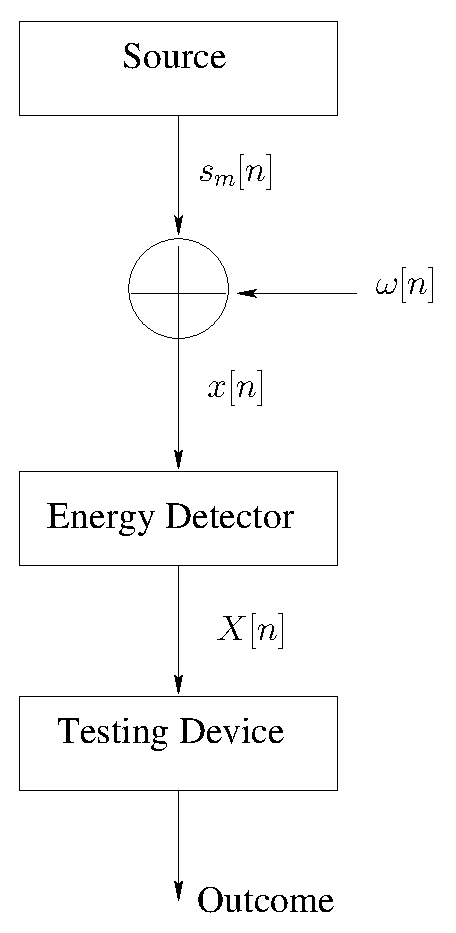
\includegraphics[width=\textwidth]{4/fig1.eps}
  \caption{Block Diagram for  cyclostationary detector.}
  \label{pic:1222a0}
\end{figure}
Like in \cite{lunden2007spectrum, lunden2010robust}, in our system the measuring device observes the noisy version of the received signals and forms an estimator of cyclic-autocorrelation (cyclic-autocorrelation is the Fourier coefficients of the signals' time-varying autocorrelation with respect to time \cite{lunden2007spectrum, lunden2010robust, dandawate1994statistical}) of their sampled version. With this statistics, the testing device employs the MENP framework to determine the status of the channel. The input of measuring device is
\begin{equation}
  \mathbf{x} = \begin{cases}
	\mathbf{n}\;\;\;\;\;\;&\text{when $H_0$ is true}\\
	\mathbf{n}+\mathbf{s}_A\;\;\;\;\;\;&\text{when $H_1$ is true}\\
	\mathbf{n}+\mathbf{s}_B\;\;\;\;\;\;&\text{when $H_2$ is true}\\
  \end{cases}
  \label{equ:1209a1}
\end{equation}
where 
\begin{equation}
  \begin{cases}
	&\mathbf{x} = (x_0, x_1, \cdots, x_{M-1})\\
	&\mathbf{s}_A = (s_{A0}, s_{A1}, \cdots, s_{A(M-1)})\\
	&\mathbf{s}_B = (s_{B0}, s_{B1}, \cdots, s_{B(M-1)})\\
	&\mathbf{n} = (n_{0}, n_{1}, \cdots, n_{M-1})\,.
  \end{cases}
  \label{xssn}
\end{equation}
Assume each OFDM frame contains a CP sequence of length $l_C$ followed by a data sequence of length $l_D$, so the total length of an OFDM frame is $l_0 = l_C+l_D$. 
From \cite{goldsmith2005wireless}, we know $l_D$ is equal to the number of subcarriers in OFDM system. 
In the general case the receiver is not synchronized to the transmitted signal, i.e. $s_{A0}$ ( or $s_{B0}$) is not the first symbol of a received OFDM frame. Let $\tau$ represents the synchronization mismatch. That is, when $\tau = 0$, $s_0$ is the first symbol of an OFDM frame; when $\tau = l_C+l_D -1$, $s_0$ is the last symbol of an OFDM frame. Let $M = Kl_0$, we can see with perfect synchronization the detector would observe $K$ complete  OFDM frames (as it is shown in Figure \ref{pic:1222ext0}); otherwise, the detector would observe $K-1$ complete OFDM frames and $2$ incomplete OFDM frames (as it is shown in Figure \ref{pic:1222a2}). 
\begin{figure}[!t]
  \centering 
  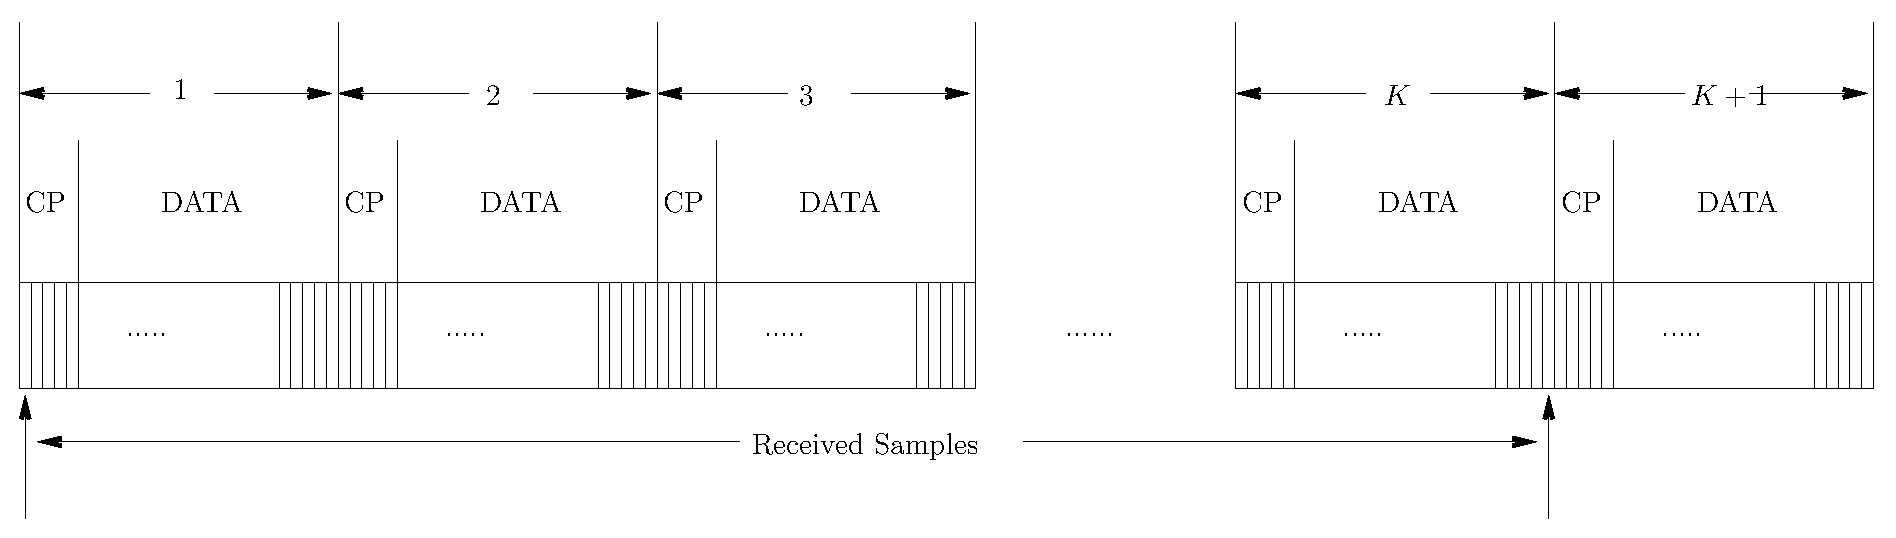
\includegraphics[width=\textwidth]{4/fig2.eps}
  \caption{Received signal for perfect synchronization.}
  \label{pic:1222ext0}
\end{figure}

\begin{figure}[!t]
  \centering 
  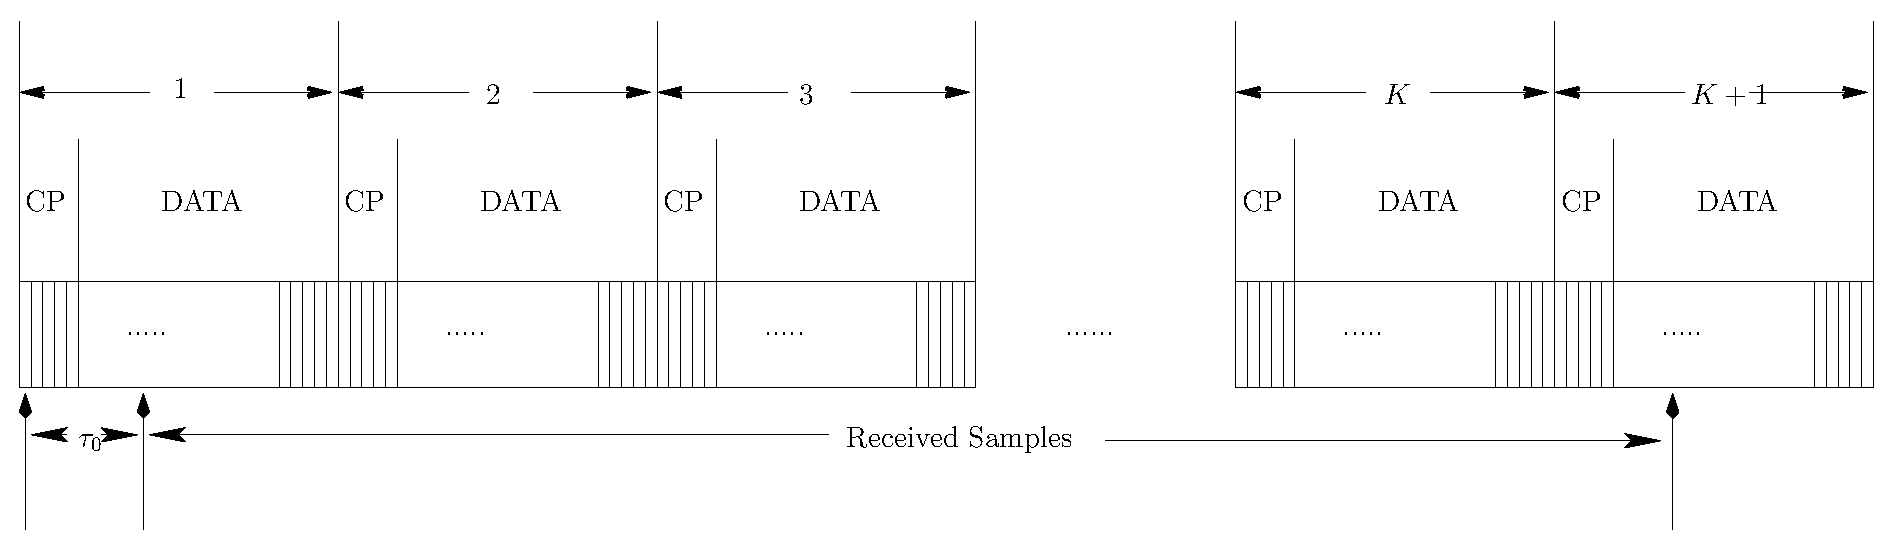
\includegraphics[width=\textwidth]{4/fig3.eps}
  \caption{Received signal for synchronization mismatch $\tau_0$.}
  \label{pic:1222a2}
\end{figure}
Assume $\tau = \tau_0$, let $\Theta_{\tau_0}$ denote the set of subscripts such that if $i \in \Theta_{\tau_0}$,  $s_i$ is a symbol of CP sequence. From Figure \ref{pic:1222ext0} we can see, in the situation of perfect synchronization ( $\tau_0 =0$), when $i \in [Ql_0, Ql_0+l_c-1]$ ($Q = 0, 1, \cdots, K-1$), the associated $s_i$ belongs to CP sequence. 
From Figure \ref{pic:1222a2}, we can see in the situation of imperfect synchronization, $i \in \Theta_{\tau_0}$ only if $i + \tau_0 \in [Ql_0, Ql_0+l_c -1]$ ($Q = 0, 1, \cdots, K-1$), i.e.
\begin{equation}
  \Theta_{\tau_0} = \{
i | i + \tau_0 \in [Ql_0, Ql_0+l_c -1], Q = 0, \cdots, K-1
  \}
\end{equation}
Let $\Theta_{\tau_0}^k$ denotes set of subscript $i$ such that  $i \in \Theta_{\tau_0}$ and $i \neq k$, i.e.
\begin{equation}
  \Theta_{\tau_0}^k =  \{i | i \in \Theta_{\tau_0} \;\;\;\; \text{and}\;\;\;\; i\neq k\}\,.
  \label{definitionoftau0k}
\end{equation}

Similar to \cite{axell2011optimal}, we make the following assumptions about the noise and signal: (1) all noise samples are i.i.d. mean zero circularly symmetric complex Gaussian (CSCG) with variance $2\sigma_n^2$, i.e. $n_i \sim \mathcal{CN}(0, 2\sigma_n)^2$; (2) when the number of subcarriers is large enough ($l_D$ is large enough), under hypothesis $H_1$ ($H_2$) the transmitted signal symbols in the data sequence are i.i.d. zero mean CSCG with variance $2\sigma_{s_A}^2$ (or $2\sigma_{s_B}^2$ under hypothesis $H_2$), i.e. $s_{Ai} \sim \mathcal{CN}(0, 2\sigma_{s_A}^2)$ $s_{Bi} \sim \mathcal{CN}(0, 2\sigma_{s_B}^2)$; (3) if $s_i$ is a sample in CP sequence, then we have $s_i = s_{i+l_D}$. 
Here we assume $\sigma_{s_A}^2$, $\sigma_{s_B}^2$ and $\sigma_n^2$  are known parameters for the detector. These parameters can be estimated as following: we first let primary user $s_A$ transmit a pilot signal (some OFDM sequence without CP structure) and estimates the variance of the received signal ($\sigma_{s_A}^2 + \sigma_n^2$). Then we let primary user $s_B$ transmit a pilot signal (some OFDM sequence without CP structure) and estimates the variance of the received signal ($\sigma_{s_B}^2 + \sigma_n^2$). In the end we stop the transmission of any primary signal to estimate the noise variance ($\sigma_n^2$). In such way we can know the variance of primary user $s_A$, $s_B$ and the noise $n$. 

Cyclostationary processes are random processes for which the statistical properties such as the mean and autocorrelation change periodically as a function of time \cite{gardner1986statistical}. 
The CP structure could introduce strong cyclostationarity to the transmitted OFDM signals ($s_A$ or $s_B$) \cite{lunden2010robust}. 
Let $r_i=x_ix_j^\ast$ ($j=i+l_D$). The moments of $\bar{r}_i, \tilde{r}_i$ are derived in \cite{axell2011optimal} and summarized in Table \ref{Table1}. 

% Please add the following required packages to your document preamble:
% \usepackage{multirow}
\begin{table}[h]
\centering
  \begin{tabular}{|c|c|c|c|c|c|}
	\hline
	\multirow{2}{*}{}           & \multirow{2}{*}{$H_0$} & \multicolumn{2}{c|}{$H_1$}                                                               & \multicolumn{2}{c|}{$H_2$}                                                               \\ \cline{3-6} 
	&                        & $i \in \Theta_{\tau_0}$                                                   & $i\notin \Theta_{\tau_0}$                          & $i\in \Theta_{\tau_0}$                                                   & $i\notin \Theta_{\tau_0}$                          \\ \hline
	$E[\bar{r}_i]$              & $0$                    & $2\sigma_{s_A}^2$                                       & $0$                            & $2\sigma_{s_B}^2$                                                         & $0$                            \\ \hline
	$E[\tilde{r}_i]$            & $0$                    & $0$                                                     & $0$                            & $0$                                                     & $0$                            \\ \hline
	$E[\bar{r}_i^2]$            & $2\sigma_n^4$          & $8\sigma_{s_A}^4+4\sigma_{s_A}^2\sigma_n^2+2\sigma_n^4$ & $2(\sigma_n^2+\sigma_{s_A}^2)^2$ & $8\sigma_{s_B}^4+4\sigma_{s_B}^2\sigma_n^2+2\sigma_n^4$ & $2(\sigma_n^2+\sigma_{s_B}^2)^2$ \\ \hline
	$E[\tilde{r}_i^2]$          & $2\sigma_n^4$          & $4\sigma_{s_A}^2\sigma_n^2+2\sigma_n^4$                 & $2(\sigma_n^2+\sigma_{s_A}^2)^2$ & $4\sigma_{s_B}^2\sigma_n^2+2\sigma_n^4$                 & $2(\sigma_n^2+\sigma_{s_B}^2)^2$ \\ \hline
	$E[\bar{r}_i\tilde{r}_i]$   & $0$                    & $0$                                                     & $0$                            & $0$                                                     & $0$                            \\ \hline
  \end{tabular}
  \caption{The moments of $r_i$}
  \label{Table1}
\end{table}

From the definition of $\Theta_{\tau_0}$ and Table \ref{Table1}, we can see under both $H_1$ or $H_2$, we have $E[s_is_j^\ast] = E[s_{i+l_0}s_{j+l_0}^\ast]$, i.e. the autocorrelation of $s_A$ or $s_B$ change periodically as a function of $i$. Hence we can conclude the OFDM signals is cyclostationary.  
\cite{lunden2007spectrum} shows that $r_i$ exhibit cyclic property at frequency $\alpha = \frac{Q}{l_0}$ ($Q = \pm1, \pm2, \cdots$) under hypotheses $H_1$ or $H_2$. In this case, to simplify our analysis, we consider a single cyclic detector at frequency $\alpha = \frac{1}{l_0}$. 
Let $\mathbf{r}$ denote the vector of $r_i$. Since the length of $\mathbf{x}$ is $M$, the length of $\mathbf{r}$ is $M - l_D$. For simple representation, let $N = M - l_D$.
Like in most related literature reviews (c.f. \cite{lunden2010robust} \cite{dandawate1994statistical}), the cyclic-autocorrelation estimator for frequency $\alpha$ can be written as
\begin{equation}
  \hat{R}(l_D, \alpha) = \frac{1}{N}\sum_{i=0}^{N-1} r_ib_i\,.
  \label{cyclicR}
\end{equation}
where $b_i = \exp(-j2\pi\alpha i)$. 
The output of the measuring device is the real and imaginary part of the cyclic-autocorrelation estimator, i.e. 
\begin{equation}
  Y = \begin{bmatrix}
	R \\
	I
  \end{bmatrix}\,,
  \label{cyclic_cov}
\end{equation}
where 
\[
  R = \Re(\hat{R}(l_D, \alpha))
\]
and 
\[
  I = \Im(\hat{R}(l_D, \alpha))\,.
\]
By observing $y$, a realization  of $Y$, the testing device determines the status of the channel.
According to \cite{lunden2010robust}, $\hat{R}(l_D, \alpha)$ has a complex normal distribution for a large $K$, so $Y$ has a two-dimensional Gaussian distribution \cite{goodman1963statistical}.
Let $\bar{c}$ and $\tilde{c}$ denote the real and imaginary parts of a complex number $c$ respectively. Then, $b_i = \bar{b}_i + j\tilde{b}_i$  and $r_i = \bar{r}_i + j\tilde{r}_i$. 


Next we compute $E[\bar{r}_i\bar{r}_k]$, $E[\bar{r}_i\tilde{r}_k]$ and $E[\tilde{r}_i\tilde{r}_k]$ when $i \neq k$ under hypothesis $H_1$. For easy presentation, let $j = i+l_D$ and $l=k+l_D$.
 The expression of $r_i$ can be written as
\begin{equation}
  \begin{split}
    r_i = &(s_i+n_i)(s_j + n_j)^\ast\\
    = &(\bar{s}_i+j\tilde{s}_i + \bar{n}_i+j\tilde{n}_i)(\bar{s}_j-j\tilde{s}_j + \bar{n}_j-j\tilde{n}_j)\\
    = &\bar{s}_i\bar{s}_j + \bar{s}_i\bar{n}_j +\tilde{s}_i\tilde{s}_j+\tilde{s}_i\tilde{n}_j + \bar{n}_i\bar{s}_j+\bar{n}_i\bar{n}_j+\tilde{n}_i\tilde{s}_j+\tilde{n}_i\tilde{n}_j\\
    + &j\left( \tilde{s}_i\bar{s}_j + \tilde{s}_i\bar{n}_j + \tilde{n}_i\bar{s}_j + \tilde{n}_i\bar{n}_j - \bar{s}_i\tilde{s}_j - \bar{s}_i\tilde{n}_j - \bar{n}_i\tilde{s}_j - \bar{n}_i\tilde{n}_j \right)
  \end{split}
\end{equation}
thus we have 
\begin{equation}
  \begin{cases}
    \bar{r}_i = \bar{s}_i\bar{s}_j + \bar{s}_i\bar{n}_j +\tilde{s}_i\tilde{s}_j+\tilde{s}_i\tilde{n}_j + \bar{n}_i\bar{s}_j+\bar{n}_i\bar{n}_j+\tilde{n}_i\tilde{s}_j+\tilde{n}_i\tilde{n}_j\\
    \tilde{r}_i = \tilde{s}_i\bar{s}_j + \tilde{s}_i\bar{n}_j + \tilde{n}_i\bar{s}_j + \tilde{n}_i\bar{n}_j - \bar{s}_i\tilde{s}_j - \bar{s}_i\tilde{n}_j - \bar{n}_i\tilde{s}_j - \bar{n}_i\tilde{n}_j\,.
  \end{cases}
  \label{RrIr}
\end{equation}

\begin{equation}
  \begin{split}
    E[\bar{r}_i\bar{r}_k] = &E[(\bar{s}_i\bar{s}_j + \bar{s}_i\bar{n}_j +\tilde{s}_i\tilde{s}_j+\tilde{s}_i\tilde{n}_j + \bar{n}_i\bar{s}_j+\bar{n}_i\bar{n}_j+\tilde{n}_i\tilde{s}_j+\tilde{n}_i\tilde{n}_j)\\
    &(\bar{s}_k\bar{s}_l + \bar{s}_k\bar{n}_l +\tilde{s}_k\tilde{s}_l+\tilde{s}_k\tilde{n}_l + \bar{n}_k\bar{s}_l+\bar{n}_k\bar{n}_l+\tilde{n}_k\tilde{s}_l+\tilde{n}_k\tilde{n}_l)]\\
    = &E[\bar{s}_j\bar{s}_k\bar{s}_i\bar{s}_l]+E[\bar{s}_j\bar{s}_k\bar{s}_i\bar{n}_l]+E[\bar{s}_j\tilde{s}_k\bar{s}_i\tilde{s}_l]+E[\bar{s}_j\tilde{s}_k\bar{s}_i\tilde{n}_l]+E[\bar{s}_j\bar{n}_k\bar{s}_i\bar{s}_l]\\
&+E[\bar{s}_j\bar{n}_k\bar{s}_i\bar{n}_l]+E[\bar{s}_j\tilde{n}_k\bar{s}_i\tilde{s}_l]+E[\bar{s}_j\tilde{n}_k\bar{s}_i\tilde{n}_l]+E[\bar{n}_j\bar{s}_i\bar{s}_l\bar{s}_k]+E[\bar{n}_j\bar{s}_i\bar{n}_l\bar{s}_k]\\
&+E[\tilde{s}_k\bar{n}_j\bar{s}_i\tilde{s}_l]+E[\tilde{s}_k\bar{n}_j\bar{s}_i\tilde{n}_l]+E[\bar{n}_j\bar{n}_k\bar{s}_i\bar{s}_l]+E[\bar{n}_j\bar{n}_k\bar{s}_i\bar{n}_l]+E[\bar{n}_j\tilde{n}_k\bar{s}_i\tilde{s}_l]\\
&+E[\bar{n}_j\tilde{n}_k\bar{s}_i\tilde{n}_l]+E[\tilde{s}_j\tilde{s}_i\bar{s}_l\bar{s}_k]+E[\tilde{s}_j\tilde{s}_i\bar{n}_l\bar{s}_k]+E[\tilde{s}_k\tilde{s}_j\tilde{s}_i\tilde{s}_l]+E[\tilde{s}_k\tilde{s}_j\tilde{s}_i\tilde{n}_l]\\
&+E[\tilde{s}_j\tilde{s}_i\bar{n}_k\bar{s}_l]+E[\tilde{s}_j\tilde{s}_i\bar{n}_k\bar{n}_l]+E[\tilde{s}_j\tilde{s}_i\tilde{n}_k\tilde{s}_l]+E[\tilde{s}_j\tilde{s}_i\tilde{n}_k\tilde{n}_l]+E[\bar{s}_k\tilde{s}_i\tilde{n}_j\bar{s}_l]\\
&+E[\bar{s}_k\tilde{s}_i\tilde{n}_j\bar{n}_l]+E[\tilde{s}_k\tilde{s}_i\tilde{n}_j\tilde{s}_l]+E[\tilde{s}_k\tilde{s}_i\tilde{n}_l\tilde{n}_j]+E[\tilde{s}_i\bar{n}_k\tilde{n}_j\bar{s}_l]+E[\tilde{s}_i\bar{n}_k\tilde{n}_j\bar{n}_l]\\
&+E[\tilde{s}_i\tilde{n}_k\tilde{n}_j\tilde{s}_l]+E[\tilde{s}_i\tilde{n}_k\tilde{n}_l\tilde{n}_j]+E[\bar{n}_i\bar{s}_j\bar{s}_l\bar{s}_k]+E[\bar{n}_i\bar{s}_j\bar{n}_l\bar{s}_k]+E[\bar{n}_i\bar{s}_j\tilde{s}_k\tilde{s}_l]\\
&+E[\bar{n}_i\bar{s}_j\tilde{n}_l\tilde{s}_k]+E[\bar{n}_i\bar{s}_j\bar{n}_k\bar{s}_l]+E[\bar{n}_i\bar{s}_j\bar{n}_k\bar{n}_l]+E[\bar{n}_i\bar{s}_j\tilde{n}_k\tilde{s}_l]+E[\bar{n}_i\bar{s}_j\tilde{n}_k\tilde{n}_l]\\
&+E[\bar{n}_i\bar{s}_k\bar{n}_j\bar{s}_l]+E[\bar{n}_i\bar{s}_k\bar{n}_j\bar{n}_l]+E[\bar{n}_i\tilde{s}_k\bar{n}_j\tilde{s}_l]+E[\bar{n}_i\tilde{s}_k\bar{n}_j\tilde{n}_l]+E[\bar{n}_i\bar{n}_k\bar{n}_j\bar{s}_l]\\
&+E[\bar{n}_i\bar{n}_k\bar{n}_j\bar{n}_l]+E[\bar{n}_i\tilde{n}_k\bar{n}_j\tilde{s}_l]+E[\bar{n}_i\tilde{n}_k\bar{n}_j\tilde{n}_l]+E[\tilde{n}_i\bar{s}_k\bar{s}_l\tilde{s}_j]+E[\tilde{n}_i\bar{n}_l\bar{s}_k\tilde{s}_j]\\
&+E[\tilde{s}_k\tilde{n}_i\tilde{s}_l\tilde{s}_j]+E[\tilde{s}_k\tilde{n}_i\tilde{n}_l\tilde{s}_j]+E[\tilde{n}_i\bar{n}_k\bar{s}_l\tilde{s}_j]+E[\tilde{n}_i\bar{n}_k\bar{n}_l\tilde{s}_j]+E[\tilde{s}_l\tilde{n}_i\tilde{n}_k\tilde{s}_j]\\
&+E[\tilde{n}_i\tilde{n}_k\tilde{n}_l\tilde{s}_j]+E[\tilde{n}_i\tilde{n}_j\bar{s}_l\bar{s}_k]+E[\tilde{n}_i\tilde{n}_j\bar{n}_l\bar{s}_k]+E[\tilde{s}_k\tilde{n}_i\tilde{n}_j\tilde{s}_l]+E[\tilde{s}_k\tilde{n}_i\tilde{n}_j\tilde{n}_l]\\
&+E[\tilde{n}_i\tilde{n}_j\bar{n}_k\bar{s}_l]+E[\tilde{n}_i\tilde{n}_j\bar{n}_k\bar{n}_l]+E[\tilde{n}_i\tilde{n}_j\tilde{n}_k\tilde{s}_l]+E[\tilde{n}_i\tilde{n}_j\tilde{n}_k\tilde{n}_l]
  \end{split}
  \label{Erij}
\end{equation}
Since noise samples are governed by i.i.d Gaussian distribution with zero mean and they are independent with signals, items in \eqref{Erij} containing noise samples would have zero value, e.g. $E[\bar{s}_j\bar{s}_k\bar{s}_i\bar{n}_l] = E[\bar{s}_j\bar{s}_k\bar{s}_i]E[\bar{n}_l] = 0$. Eliminate zero value items in equation \eqref{Erij}:
\begin{equation}
  E[\bar{r}_i\bar{r}_k] = E[\bar{s}_i\bar{s}_j\bar{s}_k\bar{s}_l] + E[\bar{s}_i\bar{s}_j\tilde{s}_k\tilde{s}_l] + E[\tilde{s}_i\tilde{s}_j\bar{s}_k\bar{s}_l] + E[\tilde{s}_i\tilde{s}_j\tilde{s}_k\tilde{s}_l]
  \label{equ:Erirk}
\end{equation} 

Without losing generality, we assume $i < k$. Consider the situation when $k \notin \Theta_{\tau_0}$, in such case $s_k$ is a symbol in data sequence so $s_k$ and $s_{k+l_D}$ are independent, i.e. $s_k$ and $s_l$ are independent. Furthermore, it is easy to see that $s_l$ is also independent of $s_i$ and $s_j$. Hence \eqref{equ:Erirk} can be written as
\begin{equation}
  \begin{split}
  E[\bar{r}_i\bar{r}_k] = &E[\bar{s}_i\bar{s}_j\bar{s}_k]E[\bar{s}_l] + E[\bar{s}_i\bar{s}_j\tilde{s}_k]E[\tilde{s}_l] + E[\tilde{s}_i\tilde{s}_j\bar{s}_k]E[\bar{s}_l] + E[\tilde{s}_i\tilde{s}_j\tilde{s}_k]E[\tilde{s}_l]\\
  = &0\,.
\end{split}
  \label{equ:Erirksitu1}
\end{equation} 
Similarly it can be proved when $i \notin \Theta_{\tau_0}$, we have $E[\bar{r}_i\bar{r}_k] =0$. Now consider the situation when $i, k \in \Theta_{\tau_0}$. In such case, we have 
\begin{equation}
  \begin{cases}
    s_i = s_j\\
    s_k = s_l
  \end{cases}
\end{equation}
and \eqref{equ:Erirk} can be written in form of
\begin{equation}
  \begin{split}
    E[\bar{r}_i\bar{r}_k] &= E[\bar{s}_i^2\bar{s}_k^2] + E[\bar{s}_i^2\tilde{s}_k^2]  +E[\tilde{s}_i^2\bar{s}_k^2] + E[\tilde{s}_i^2\tilde{s}_k^2] \\
    &= E[\bar{s}_i^2]E[\bar{s}_k^2] + E[\bar{s}_i^2]E[\tilde{s}_k^2]  +E[\tilde{s}_i^2]E[\bar{s}_k^2] + E[\tilde{s}_i^2]E[\tilde{s}_k^2] \\
    &= 4\sigma_{s_A}^4\,.
  \end{split}
  \label{Eririsitu2}
\end{equation}

From above discussion, the value of $E[\bar{r}_i\bar{r}_k]$  ($i \neq k$) can be summarized as
\begin{equation}
  E[\bar{r}_i\bar{r}_k] =  \begin{cases}
    4\sigma_{s_A}^4 \;\;\;\;&i, k \in \Theta_{\tau_0}\\
    0\;\;\;\;&\text{Otherwise}
  \end{cases}
  \label{Er_ir_j}
\end{equation}

Next consider $E[\bar{r}_i\tilde{r}_j]$, which can be written as
\begin{equation}
  \begin{split}
E[\bar{r}_i\tilde{r}_j] = &E[(\bar{s}_i\bar{s}_j + \bar{s}_i\bar{n}_j +\tilde{s}_i\tilde{s}_j+\tilde{n}_i\tilde{n}_j + \bar{n}_i\bar{s}_j+\bar{n}_i\bar{n}_j+\tilde{n}_i\tilde{s}_j+\tilde{n}_i\tilde{n}_j)\\
              &(\tilde{s}_k\bar{s}_l + \tilde{s}_k\bar{n}_l + \tilde{n}_k\bar{s}_l + \tilde{n}_k\bar{n}_l - \bar{s}_k\tilde{s}_l - \bar{s}_k\tilde{n}_l - \bar{n}_k\tilde{s}_l - \bar{n}_k\tilde{n}_l)]\,.
%              = &E[\bar{s}_j\tilde{s}_k\bar{s}_i\bar{s}_l]+E[\bar{s}_j\tilde{s}_k\bar{s}_i\bar{n}_l]+E[\bar{s}_j\tilde{n}_k\bar{s}_i\bar{s}_l]+E[\bar{s}_j\tilde{n}_k\bar{s}_i\bar{n}_l]-E[\bar{s}_j\bar{s}_k\bar{s}_i\tilde{s}_l]\\
%&-E[\bar{s}_j\bar{s}_k\bar{s}_i\tilde{n}_l]-E[\bar{s}_j\bar{n}_k\bar{s}_i\tilde{s}_l]-E[\bar{s}_j\bar{n}_k\bar{s}_i\tilde{n}_l]+E[\tilde{s}_k\bar{n}_j\bar{s}_i\bar{s}_l]+E[\tilde{s}_k\bar{n}_j\bar{s}_i\bar{n}_l]\\
%&+E[\bar{n}_j\tilde{n}_k\bar{s}_i\bar{s}_l]+E[\bar{n}_j\tilde{n}_k\bar{s}_i\bar{n}_l]-E[\tilde{s}_l\bar{n}_j\bar{s}_i\bar{s}_k]-E[\bar{n}_j\bar{s}_i\tilde{n}_l\bar{s}_k]-E[\bar{n}_j\bar{n}_k\bar{s}_i\tilde{s}_l]\\
%&-E[\bar{n}_j\bar{n}_k\bar{s}_i\tilde{n}_l]+E[\tilde{s}_k\tilde{s}_j\tilde{s}_i\bar{s}_l]+E[\tilde{s}_k\tilde{s}_j\tilde{s}_i\bar{n}_l]+E[\tilde{s}_j\tilde{s}_i\tilde{n}_k\bar{s}_l]+E[\tilde{s}_j\tilde{s}_i\tilde{n}_k\bar{n}_l]\\
%&-E[\tilde{s}_j\tilde{s}_i\tilde{s}_l\bar{s}_k]-E[\tilde{s}_j\tilde{s}_i\tilde{n}_l\bar{s}_k]-E[\tilde{s}_j\tilde{s}_i\bar{n}_k\tilde{s}_l]-E[\tilde{s}_j\tilde{s}_i\tilde{n}_l\bar{n}_k]+E[\tilde{s}_k\tilde{n}_i\tilde{n}_j\bar{s}_l]\\
%&+E[\tilde{s}_k\tilde{n}_i\tilde{n}_j\bar{n}_l]+E[\tilde{n}_i\tilde{n}_j\tilde{n}_k\bar{s}_l]+E[\tilde{n}_i\tilde{n}_j\tilde{n}_k\bar{n}_l]-E[\tilde{n}_i\tilde{n}_j\tilde{s}_l\bar{s}_k]-E[\tilde{n}_i\tilde{n}_j\tilde{n}_l\bar{s}_k]\\
%&-E[\tilde{n}_i\tilde{n}_j\bar{n}_k\tilde{s}_l]-E[\tilde{n}_i\tilde{n}_j\tilde{n}_l\bar{n}_k]+E[\bar{n}_i\bar{s}_j\bar{s}_l\tilde{s}_k]+E[\bar{n}_i\bar{s}_j\bar{n}_l\tilde{s}_k]+E[\bar{n}_i\bar{s}_j\tilde{n}_k\bar{s}_l]\\
%&+E[\bar{n}_i\bar{s}_j\tilde{n}_k\bar{n}_l]-E[\bar{n}_i\bar{s}_j\tilde{s}_l\bar{s}_k]-E[\bar{n}_i\bar{s}_j\tilde{n}_l\bar{s}_k]-E[\bar{n}_i\bar{s}_j\bar{n}_k\tilde{s}_l]-E[\bar{n}_i\bar{s}_j\bar{n}_k\tilde{n}_l]\\
%&+E[\bar{n}_i\tilde{s}_k\bar{n}_j\bar{s}_l]+E[\bar{n}_i\tilde{s}_k\bar{n}_j\bar{n}_l]+E[\bar{n}_i\tilde{n}_k\bar{n}_j\bar{s}_l]+E[\bar{n}_i\tilde{n}_k\bar{n}_j\bar{n}_l]-E[\bar{n}_i\bar{s}_k\bar{n}_j\tilde{s}_l]\\
%&-E[\bar{n}_i\bar{s}_k\bar{n}_j\tilde{n}_l]-E[\bar{n}_i\bar{n}_k\bar{n}_j\tilde{s}_l]-E[\bar{n}_i\bar{n}_k\bar{n}_j\tilde{n}_l]+E[\tilde{s}_k\tilde{n}_i\bar{s}_l\tilde{s}_j]+E[\tilde{s}_k\tilde{n}_i\bar{n}_l\tilde{s}_j]\\
%&+E[\tilde{n}_i\tilde{n}_k\bar{s}_l\tilde{s}_j]+E[\tilde{n}_i\tilde{n}_k\bar{n}_l\tilde{s}_j]-E[\tilde{n}_i\tilde{s}_l\bar{s}_k\tilde{s}_j]-E[\tilde{n}_i\tilde{n}_l\bar{s}_k\tilde{s}_j]-E[\tilde{n}_i\bar{n}_k\tilde{s}_l\tilde{s}_j]\\
%&-E[\tilde{n}_i\bar{n}_k\tilde{n}_l\tilde{s}_j]+E[\tilde{s}_k\tilde{n}_i\tilde{n}_j\bar{s}_l]+E[\tilde{s}_k\tilde{n}_i\tilde{n}_j\bar{n}_l]+E[\tilde{n}_i\tilde{n}_j\tilde{n}_k\bar{s}_l]+E[\tilde{n}_i\tilde{n}_j\tilde{n}_k\bar{n}_l]\\
%&-E[\tilde{n}_i\tilde{n}_j\tilde{s}_l\bar{s}_k]-E[\tilde{n}_i\tilde{n}_j\tilde{n}_l\bar{s}_k]-E[\tilde{n}_i\tilde{n}_j\bar{n}_k\tilde{s}_l]-E[\tilde{n}_i\tilde{n}_j\tilde{n}_l\bar{n}_k]
\end{split}
\label{Eriiiirk}
\end{equation}
Expanding \eqref{Eriiiirk} and eliminating the zero value items (items including noise samples), we have 
 \begin{equation}
   E[\bar{r}_i\tilde{r}_k] = E[\bar{s}_j\tilde{s}_k\bar{s}_i\bar{s}_l] -  E[\bar{s}_j\bar{s}_k\bar{s}_i\tilde{s}_l] + E[\tilde{s}_j\tilde{s}_k\tilde{s}_i\bar{s}_l] - E[\tilde{s}_j\bar{s}_k\tilde{s}_i\tilde{s}_l]\,.
   \label{equ:1213a}
\end{equation}
Since the real and imaginary part of transmitted OFDM signals are independent and $E[\bar{s}_m] = E[\tilde{s}_m] = 0$ ($m = 0, 1, \cdots, N$), \eqref{equ:1213a} can be written as
\begin{equation}
  \begin{split}
  E[\bar{r}_i\tilde{r}_k] &= E[\tilde{s}_k]E[\bar{s}_i\bar{s}_j\bar{s}_l]  - E[\tilde{s}_l]E[\bar{s}_i\bar{s}_j\bar{s}_k] + E[\bar{s}_l]E[\tilde{s}_i\tilde{s}_j\tilde{s}_k] -  E[\bar{s}_k]E[\tilde{s}_i\tilde{s}_j\tilde{s}_l]\\
  &= 0
\end{split}
  \label{equ:1215m}
\end{equation}
thus we can see $E[\bar{r}_i\tilde{r}_k] = 0$  when $i \neq k $.  

Next consider $E[\tilde{r}_i\tilde{r}_k]$, which can be written as
\begin{equation}
  \begin{split}
    E[\tilde{r}_i\tilde{r}_k] = &E[(\tilde{s}_i\bar{s}_j + \tilde{s}_i\bar{n}_j + \tilde{n}_i\bar{s}_j + \tilde{n}_i\bar{n}_j - \bar{s}_i\tilde{s}_j - \bar{s}_i\tilde{n}_j - \bar{n}_i\tilde{s}_j - \bar{n}_i\tilde{n}_j)\\
    &(\tilde{s}_k\bar{s}_l + \tilde{s}_k\bar{n}_l + \tilde{n}_k\bar{s}_l + \tilde{n}_k\bar{n}_l - \bar{s}_k\tilde{s}_l - \bar{s}_k\tilde{n}_l - \bar{n}_k\tilde{s}_l - \bar{n}_k\tilde{n}_l)]
%    = &E[\bar{s}_j\tilde{s}_k\tilde{s}_i\bar{s}_l]+E[\bar{s}_j\tilde{s}_k\tilde{s}_i\bar{n}_l]+E[\bar{s}_j\tilde{s}_i\tilde{n}_k\bar{s}_l]+E[\bar{s}_j\tilde{s}_i\tilde{n}_k\bar{n}_l]-E[\bar{s}_j\bar{s}_k\tilde{s}_i\tilde{s}_l]\\
%&-E[\bar{s}_j\bar{s}_k\tilde{s}_i\tilde{n}_l]-E[\bar{s}_j\tilde{s}_i\bar{n}_k\tilde{s}_l]-E[\bar{s}_j\tilde{s}_i\tilde{n}_l\bar{n}_k]+E[\tilde{s}_k\tilde{s}_i\bar{n}_j\bar{s}_l]+E[\tilde{s}_k\tilde{s}_i\bar{n}_j\bar{n}_l]\\
%&+E[\tilde{n}_k\tilde{s}_i\bar{n}_j\bar{s}_l]+E[\tilde{n}_k\tilde{s}_i\bar{n}_j\bar{n}_l]-E[\bar{s}_k\tilde{s}_i\bar{n}_j\tilde{s}_l]-E[\bar{s}_k\tilde{s}_i\bar{n}_j\tilde{n}_l]-E[\tilde{s}_i\bar{n}_j\bar{n}_k\tilde{s}_l]\\
%&-E[\tilde{s}_i\bar{n}_j\tilde{n}_l\bar{n}_k]+E[\bar{s}_j\tilde{n}_i\bar{s}_l\tilde{s}_k]+E[\bar{s}_j\tilde{n}_i\bar{n}_l\tilde{s}_k]+E[\bar{s}_j\tilde{n}_i\tilde{n}_k\bar{s}_l]+E[\bar{s}_j\tilde{n}_i\tilde{n}_k\bar{n}_l]\\
%&-E[\bar{s}_j\tilde{n}_i\tilde{s}_l\bar{s}_k]-E[\bar{s}_j\tilde{n}_i\tilde{n}_l\bar{s}_k]-E[\bar{s}_j\tilde{n}_i\bar{n}_k\tilde{s}_l]-E[\bar{s}_j\tilde{n}_i\bar{n}_k\tilde{n}_l]+E[\tilde{s}_k\tilde{n}_i\bar{n}_j\bar{s}_l]\\
%&+E[\tilde{s}_k\tilde{n}_i\bar{n}_j\bar{n}_l]+E[\tilde{n}_i\tilde{n}_k\bar{n}_j\bar{s}_l]+E[\tilde{n}_i\tilde{n}_k\bar{n}_j\bar{n}_l]-E[\tilde{s}_l\tilde{n}_i\bar{n}_j\bar{s}_k]-E[\tilde{n}_i\bar{n}_j\tilde{n}_l\bar{s}_k]\\
%&-E[\tilde{n}_i\bar{n}_k\bar{n}_j\tilde{s}_l]-E[\tilde{n}_i\bar{n}_k\bar{n}_j\tilde{n}_l]-E[\tilde{s}_k\tilde{s}_j\bar{s}_i\bar{s}_l]-E[\tilde{s}_k\tilde{s}_j\bar{s}_i\bar{n}_l]-E[\tilde{s}_j\tilde{n}_k\bar{s}_i\bar{s}_l]\\
%&-E[\tilde{s}_j\tilde{n}_k\bar{s}_i\bar{n}_l]+E[\tilde{s}_l\tilde{s}_j\bar{s}_i\bar{s}_k]+E[\tilde{s}_j\bar{s}_i\tilde{n}_l\bar{s}_k]+E[\tilde{s}_j\bar{n}_k\bar{s}_i\tilde{s}_l]+E[\tilde{s}_j\bar{n}_k\bar{s}_i\tilde{n}_l]\\
%&-E[\tilde{s}_k\tilde{n}_j\bar{s}_i\bar{s}_l]-E[\tilde{s}_k\tilde{n}_j\bar{s}_i\bar{n}_l]-E[\tilde{n}_k\tilde{n}_j\bar{s}_i\bar{s}_l]-E[\tilde{n}_k\tilde{n}_j\bar{s}_i\bar{n}_l]+E[\bar{s}_k\tilde{n}_j\bar{s}_i\tilde{s}_l]\\
%&+E[\bar{s}_k\tilde{n}_j\bar{s}_i\tilde{n}_l]+E[\tilde{n}_j\bar{s}_i\bar{n}_k\tilde{s}_l]+E[\tilde{n}_j\bar{s}_i\tilde{n}_l\bar{n}_k]-E[\bar{n}_i\tilde{s}_j\bar{s}_l\tilde{s}_k]-E[\bar{n}_i\tilde{s}_j\bar{n}_l\tilde{s}_k]\\
%&-E[\bar{n}_i\tilde{s}_j\tilde{n}_k\bar{s}_l]-E[\bar{n}_i\tilde{s}_j\tilde{n}_k\bar{n}_l]+E[\bar{n}_i\tilde{s}_j\tilde{s}_l\bar{s}_k]+E[\bar{n}_i\tilde{s}_j\tilde{n}_l\bar{s}_k]+E[\bar{n}_i\tilde{s}_j\bar{n}_k\tilde{s}_l]\\
%&+E[\bar{n}_i\tilde{s}_j\bar{n}_k\tilde{n}_l]-E[\bar{n}_i\tilde{s}_k\tilde{n}_j\bar{s}_l]-E[\bar{n}_i\tilde{s}_k\tilde{n}_j\bar{n}_l]-E[\bar{n}_i\tilde{n}_j\tilde{n}_k\bar{s}_l]-E[\bar{n}_i\tilde{n}_j\tilde{n}_k\bar{n}_l]\\
%&+E[\bar{n}_i\bar{s}_k\tilde{n}_j\tilde{s}_l]+E[\bar{n}_i\bar{s}_k\tilde{n}_j\tilde{n}_l]+E[\bar{n}_i\tilde{n}_j\bar{n}_k\tilde{s}_l]+E[\bar{n}_i\tilde{n}_j\tilde{n}_l\bar{n}_k]
  \end{split}
  \label{EEEErrrrr}
\end{equation}
Expanding \eqref{EEEErrrrr} and eliminating the zero value items (items including noise samples), we have 
\begin{equation}
  E[\tilde{r}_i\tilde{r}_k] = E[\bar{s}_j\tilde{s}_k\tilde{s}_i\bar{s}_l] -  E[\bar{s}_j\bar{s}_k\tilde{s}_i\tilde{s}_l] - E[\tilde{s}_j\tilde{s}_k\bar{s}_i\bar{s}_l] +E[\tilde{s}_j\bar{s}_k\bar{s}_i\tilde{s}_l]
  \label{1213night}
\end{equation}

Similar to $E[\bar{r}_i\bar{r}_k]$, when $i$ (or $k$) does not belong to set $\Theta_{\tau_0}$, we can see
that $   E[\tilde{r}_i\tilde{r}_k] = 0$.

When $i, k \in \Theta_{\tau_0}$, equation \eqref{1213night} can be written as
\begin{equation}
  \begin{split}
  E[\tilde{r}_i\tilde{r}_k] = &E[\bar{s}_i\tilde{s}_k\tilde{s}_i\bar{s}_k] -  E[\bar{s}_i\bar{s}_k\tilde{s}_i\tilde{s}_k] - E[\tilde{s}_i\tilde{s}_k\bar{s}_i\bar{s}_k] +E[\tilde{s}_i\bar{s}_k\bar{s}_i\tilde{s}_k]\\
  = &E[\bar{s}_i]E[\tilde{s}_k]E[\tilde{s}_i]E[\bar{s}_k] -  E[\bar{s}_i]E[\bar{s}_k]E[\tilde{s}_i]E[\tilde{s}_k] - E[\tilde{s}_i]E[\tilde{s}_k]E[\bar{s}_i]E[\bar{s}_k] +E[\tilde{s}_i]E[\bar{s}_k]E[\bar{s}_i]E[\tilde{s}_k]\\
  = &0\,.
  \end{split}
\end{equation}
Hence we can conclude $E[\tilde{r}_i\tilde{r}_k] = 0$ when $i \neq k$. 

The statistics of $E[\bar{r}_i\bar{r}_k]$, $E[\bar{r}_i\tilde{r}_k]$ and $E[\tilde{r}_i\tilde{r}_k]$ under hypothesis $H_1$ are summarized in Table \ref{Table3}. 
\begin{table}[h]
\centering
\begin{tabular}{|c|c|c|c|c|}
\hline
\multirow{2}{*}{Statistics} & \multicolumn{2}{c|}{$i = k$}                                                              & \multicolumn{2}{c|}{$i \neq k$}        \\ \cline{2-5} 
                            & $i\in \Theta_{\tau_0}$                                 & $i \notin \Theta_{\tau_0}$       & $i, k \in \Theta_{\tau_0}$ & Otherwise  \\ \hline
$E[\bar{r}_i\bar{r}_k]$     & $8\sigma_{s_A}^4+4\sigma_{s_A}^2\sigma_n^2+2\sigma_n^4$ & $2(\sigma_n^2+\sigma_{s_A}^2)^2$ & $4\sigma_{s_A}^4$          & $0$       \\ \hline
$E[\bar{r}_i\tilde{r}_k]$   & $0$                                                    & $0$                              & $0$                        & $0$       \\ \hline
$E[\tilde{r}_i\tilde{r}_k]$ & $4\sigma_{s_A}^2\sigma_n^2+2\sigma_n^4$                & $2(\sigma_n^2+\sigma_{s_A}^2)^2$ & $0$                        & $0$       \\ \hline
\end{tabular}
\caption{$E[\bar{r}_i\bar{r}_k]$, $E[\bar{r}_i\tilde{r}_k]$ and $E[\tilde{r}_i\tilde{r}_k]$ under hypothesis $H_1$}
\label{Table3}
\end{table}

In the following, we consider the distribution of $\begin{bmatrix}
  R \\
  I
\end{bmatrix}$ under hypothesis $H_1$ with synchronization mismatch $\tau = \tau_0$.
From the definition of $R$ and $I$, we have 
\begin{equation}
  \begin{split}
	R = &\Re{(\frac{1}{N}\sum_{i=0}^{N-1} b_ir_i)}\\
	= &\Re(\frac{1}{N}\sum_{i=0}^{N-1}(\bar{b}_i+j\tilde{b}_i)(\bar{r}_i+j\tilde{r}_i))\\
	= &\frac{1}{N}\sum_{i=0}^{N-1}\bar{b}_i\bar{r}_i - \frac{1}{N}\sum_{i=0}^{N-1}\tilde{b}_i\tilde{r}_i
  \end{split}
  \label{R}
\end{equation}
and
\begin{equation}
  \begin{split}
	I = &\Im(\frac{1}{N}\sum_{i=0}^{N-1} b_ir_i)\\
	= &\frac{1}{N}\sum_{i=0}^{N-1}\tilde{b}_i\bar{r}_i + \frac{1}{N}\sum_{i=0}^{N-1}\bar{b}_i\tilde{r}_i
  \end{split}
  \label{I}
\end{equation}

Let $a_i = \frac{1}{N}b_i$, then we have 
\begin{equation}
  \begin{cases}
	&R = \sum_{i=0}^{N-1}\bar{a}_i\bar{r}_i - \sum_{i=0}^{N-1}\tilde{a}_i\tilde{r}_i\\
	&I = \sum_{i=0}^{N-1}\tilde{a}_i\bar{r}_i +\sum_{i=0}^{N-1}\bar{a}_i\tilde{r}_i\,.
  \end{cases}
  \label{definitionofRI}
\end{equation}

Let $\mu_{AR|\tau_0}$ $\mu_{AI|\tau_0}$ denote the mean of $R$ and $I$ with synchronization mismatch $\tau=\tau_0$ respectively. By using the statistics of $r_i$ from Table \ref{Table1}, we compute  $\mu_{AR|\tau_0}$ and  $\mu_{AI|\tau_0}$:
\begin{equation}
  \begin{split}
	\mu_{AR|\tau_0} =  E[R] = &\sum_{i=0}^{N-1}\bar{a}_iE[\bar{r}_i] - \sum_{i=0}^{N-1}\tilde{a}_iE[\tilde{r}_i]\\
	= &\sum_{i\in\Theta_{\tau_0}}\bar{a}_iE[\bar{r}_i]\\
	= &2\sigma_{s_A}^2\sum_{i\in\Theta_{\tau_0}}\bar{a}_i
  \end{split}
  \label{ER}
\end{equation}

\begin{equation}
  \begin{split}
	\mu_{AI|\tau_0} =  E[I] = &\sum_{i=0}^{N-1}\tilde{a}_iE[\bar{r}_i] + \sum_{i=0}^{N-1}\bar{a}_iE[\tilde{r}_i]\\
	= &\sum_{i\in\Theta_{\tau_0}}\tilde{a}_iE[\bar{r}_i]\\
    = &2\sigma_{s_A}^2\sum_{i\in\Theta_{\tau_0}}\tilde{a}_i\,.
  \end{split}
  \label{EI}
\end{equation}

The  second order statistic of $R$ and $I$ can be computed as
\begin{equation}
  \begin{split}
	E[R^2] = &E[(\sum_{i=0}^{N-1}\bar{a}_i\bar{r}_i - \sum_{i=0}^{N-1}\tilde{a}_i\tilde{r}_i)(\sum_{i=0}^{N-1}\bar{a}_i\bar{r}_i - \sum_{i=0}^{N-1}\tilde{a}_i\tilde{r}_i)]\\
	= &E[\sum_{i=0}^{N-1}\sum_{k=0}^{N-1}\bar{a}_i\bar{a}_k\bar{r}_i\bar{r}_k - \sum_{i=0}^{N-1}\sum_{k=0}^{N-1}\bar{a}_i\tilde{a}_k\bar{r}_i\tilde{r}_k - \sum_{i=0}^{N-1}\sum_{k=0}^{N-1}\bar{a}_i\tilde{a}_k\bar{r}_i\tilde{r}_k + \sum_{i=0}^{N-1}\sum_{k=0}^{N-1}\tilde{a}_i\tilde{a}_k\tilde{r}_i\tilde{r}_k]\\
	= &\sum_{i=0}^{N-1}\sum_{k=0}^{N-1}\bar{a}_i\bar{a}_kE[\bar{r}_i\bar{r}_k] - \sum_{i=0}^{N-1}\sum_{k=0}^{N-1}\bar{a}_i\tilde{a}_kE[\bar{r}_i\tilde{r}_k] - \sum_{i=0}^{N-1}\sum_{k=0}^{N-1}\bar{a}_i\tilde{a}_kE[\bar{r}_i\tilde{r}_k] + \sum_{i=0}^{N-1}\sum_{k=0}^{N-1}\tilde{a}_i\tilde{a}_kE[\tilde{r}_i\tilde{r}_k]\,.
  \end{split}
  \label{ER^2}
 \end{equation}
 From Table \ref{Table3}, we can see $E[\bar{r}_i\bar{r}_k]$ is not equal to zero when one of following two situations is satisfied: (1) $i = k$; (2) $i, k \in \Theta_{\tau_0}$ and $i \neq k$. Hence we have 
 \[
\sum_{i=0}^{N-1}\sum_{k=0}^{N-1}\bar{a}_i\bar{a}_kE[\bar{r}_i\bar{r}_k] = 
\sum_{i=0}^{N-1}\bar{a}_i^2E[\bar{r}_i^2] + \sum_{i\in\Theta_{\tau_0}}\sum_{k\in\Theta_{\tau_0}^i}\bar{a}_i\bar{a}_kE[\bar{r}_i\bar{r}_k]
 \]
 where $\Theta_{\tau_0}^i$ is defined in \eqref{definitionoftau0k}. 
 According to whether or not $i \in \Theta_{\tau_0}$,  $\sum_{i=0}^{N-1}\bar{a}_i^2E[\bar{r}_i^2]$  can be written as
 \[
\sum_{i=0}^{N-1}\bar{a}_i^2E[\bar{r}_i^2]=
\sum_{i\in\Theta_{\tau_0}}\bar{a}_i^2E[\bar{r}_i^2] + \sum_{i\notin\Theta_{\tau_0}}\bar{a}_i^2E[\bar{r}_i^2]
 \]
leads to 
\begin{equation}
\sum_{i=0}^{N-1}\sum_{k=0}^{N-1}\bar{a}_i\bar{a}_kE[\bar{r}_i\bar{r}_k] = 
\sum_{i\in\Theta_{\tau_0}}\bar{a}_i^2E[\bar{r}_i^2] + \sum_{i\notin\Theta_{\tau_0}}\bar{a}_i^2E[\bar{r}_i^2] + \sum_{i\in\Theta_{\tau_0}}\sum_{k\in\Theta_{\tau_0}^i}\bar{a}_i\bar{a}_kE[\bar{r}_i\bar{r}_k]
  \label{equ:2015may04a0}
\end{equation}
Similarly, from Table \ref{Table3} we have
 \begin{equation}
   E[\bar{r}_i\tilde{r}_k]= 0 
   \label{equ:2015may04a1}
 \end{equation}
and
\begin{equation}
  \begin{split}
\sum_{i=0}^{N-1}\sum_{k=0}^{N-1}\tilde{a}_i\tilde{a}_kE[\tilde{r}_i\tilde{r}_k]  =&  \sum_{i=0}^{N-1}\tilde{a}_i^2E[\tilde{r}_i^2]\\
=& \sum_{i\in\Theta_{\tau_0}}\tilde{a}_i^2E[\tilde{r}_i^2] + \sum_{i\notin\Theta_{\tau_0}}\tilde{a}_i^2E[\tilde{r}_i^2]
  \end{split}
  \label{equ:2015may04a2}
\end{equation}

Substituting \eqref{equ:2015may04a0}, \eqref{equ:2015may04a1} and \eqref{equ:2015may04a2} into \eqref{ER^2} leads to 
 \begin{equation}
  \begin{split}
	E[R^2]  
    = &(\sum_{i\in\Theta_{\tau_0}}\bar{a}_i^2E[\bar{r}_i^2] + \sum_{i\notin\Theta_{\tau_0}}\bar{a}_i^2E[\bar{r}_i^2]  + \sum_{i\in\Theta_{\tau_0}}\sum_{k\in\Theta_{\tau_0}^i}\bar{a}_i\bar{a}_kE[\bar{r}_i\bar{r}_k]) + (\sum_{i\in\Theta_{\tau_0}}\tilde{a}_i^2E[\tilde{r}_i^2] + \sum_{i\notin\Theta_{\tau_0}}\tilde{a}_i^2E[\tilde{r}_i^2]) \\
	= &\sum_{i\in\Theta_{\tau_0}}\bar{a}_i^2E[\bar{r}_i^2] + \sum_{i\in\Theta_{\tau_0}}\tilde{a}_i^2E[\tilde{r}_i^2] + \sum_{i\notin\Theta_{\tau_0}}(\bar{a}_i^2E[\bar{r}_i^2]+\tilde{a}_i^2E[\tilde{r}_i^2]) + \sum_{i\in\Theta_{\tau_0}}\sum_{k\in\Theta_{\tau_0}^i}\bar{a}_i\bar{a}_kE[\bar{r}_i\bar{r}_k]\\
	= &\sum_{i\in\Theta_{\tau_0}}\bar{a}_i^2(8\sigma_{s_A}^4+4\sigma_{s_A}^2\sigma_n^2+2\sigma_n^4) + \sum_{i\in\Theta_{\tau_0}}\tilde{a}_i^2(4\sigma_{s_A}^2\sigma_n^2+2\sigma_n^4) + \sum_{i\notin\Theta_{\tau_0}}(\tilde{a}_i^2+\bar{a}_i^2)2(\sigma_n^2+\sigma_{s_A}^2)^2\\
    &+4\sigma_{s_A}^4\sum_{i\in\Theta_{\tau_0}}\sum_{k\in\Theta_{\tau_0}^i}\bar{a}_i\bar{a}_k\\
  = & \sum_{i\in\Theta_{\tau_0}}(\tilde{a}_i^2 + \bar{a}_i^2)(4\sigma_{s_A}^2\sigma_n^2+2\sigma_n^4)+ \sum_{i\in\Theta_{\tau_0}}\bar{a}_i^2 8\sigma_{s_A}^4 + \sum_{i\notin\Theta_{\tau_0}}(\tilde{a}_i^2+\bar{a}_i^2)2(\sigma_n^2+\sigma_{s_A}^2)^2\\
    &+4\sigma_{s_A}^4\sum_{i\in\Theta_{\tau_0}}\sum_{k\in\Theta_{\tau_0}^i}\bar{a}_i\bar{a}_k
  \end{split}
  \label{2015apr25a0}
\end{equation}
From the definition of $a_i$ and $b_i$, we have
\begin{equation}
  \bar{a}_i^2 + \tilde{a}_i^2 =\frac{1}{N^2}
  \label{aisquare}
\end{equation}
hence \eqref{2015apr25a0} can be written as
\begin{equation}
  \begin{split}
	E[R^2] = &\frac{1}{N^2}\sum_{i\in\Theta_{\tau_0}}  (4\sigma_{s_A}^2\sigma_n^2+2\sigma_n^4)+ 8\sum_{i\in\Theta_{\tau_0}}\bar{a}_i^2\sigma_{s_A}^4 + \frac{2}{N^2}\sum_{i\notin\Theta_{\tau_0}}(\sigma_n^2+\sigma_{s_A}^2)^2 + 4\sigma_{s_A}^4\sum_{i\in\Theta_{\tau_0}}\sum_{k\in\Theta_{\tau_0}^i}\bar{a}_i\bar{a}_k\\
	= &\frac{1}{N^2}|\Theta_{\tau_0}|(4\sigma_{s_A}^2\sigma_n^2+2\sigma_n^4) +  8\sigma_{s_A}^4\sum_{i\in\Theta_{\tau_0}}\bar{a}_i^2+ \frac{2}{N^2}(N - |\Theta_{\tau_0}|)(\sigma_n^2+\sigma_{s_A}^2)^2\\
    &+4\sigma_{s_A}^4\sum_{i\in\Theta_{\tau_0}}\sum_{k\in\Theta_{\tau_0}^i}\bar{a}_i\bar{a}_k
  \end{split}
  \label{ER2}
\end{equation}
where $|\Theta_{\tau_0}|$ is the cardinality of set $\Theta_{\tau_0}$. 
Let $\sigma_{AR|\tau_0}$ $\sigma_{AI|\tau_0}$ denote the standard deviation of $R$ and $I$ when the synchronization mismatch is $\tau_0$. Then 
\begin{equation}
  \begin{split}
	\sigma_{AR|\tau_0} = &\sqrt{E[R^2] - E[R]^2}\\
	= &\left(\frac{1}{N^2}|\Theta_{\tau_0}|(4\sigma_{s_A}^2\sigma_n^2+2\sigma_n^4) + \frac{2}{N^2}(N - |\Theta_{\tau_0}|)(\sigma_n^2+\sigma_{s_A}^2)^2 +  8\sigma_{s_A}^4\sum_{i\in\Theta_{\tau_0}}\bar{a}_i^2 \right.\\
  &\left.+ 4\sigma_{s_A}^4\sum_{i\in\Theta_{\tau_0}}\sum_{k\in\Theta_{\tau_0}^i}\bar{a}_i\bar{a}_k- \mu_{AR|\tau_0}^2\right)^\frac{1}{2}\,.
  \end{split}
  \label{deviationR}
\end{equation}
Let $\beta_{\tau_0}^A = \frac{1}{N^2}|\Theta_{\tau_0}|(4\sigma_{s_A}^2\sigma_n^2+2\sigma_n^4) + \frac{2}{N^2}(N - |\Theta_{\tau_0}|)(\sigma_n^2+\sigma_{s_A}^2)^2$. Then the above equation can be written as
\begin{equation}
  \sigma_{AR|\tau_0} = \left(\beta_{\tau_0}^A+  8\sigma_{s_A}^4\sum_{i\in\Theta_{\tau_0}}\bar{a}_i^2 
    + 4\sigma_{s_A}^4\sum_{i\in\Theta_{\tau_0}}\sum_{k\in\Theta_{\tau_0}^i}\bar{a}_i\bar{a}_k- \mu_{AR|\tau_0}^2\right)^\frac{1}{2}\,.
  \label{devR}
\end{equation}

Similarly, we compute $\sigma_{AI|\tau_0}$ and $E[RI]$ as
\begin{equation}
  \begin{split}
	E[I^2] = &E[(\sum_{i=0}^{N-1}\tilde{a}_i\bar{r}_i + \sum_{i=0}^{N-1}\bar{a}_i\tilde{r}_i)(\sum_{i=0}^{N-1}\tilde{a}_i\bar{r}_i + \sum_{i=0}^{N-1}\bar{a}_i\tilde{r}_i)]\\
	= &\sum_{i=0}^{N-1}\sum_{k=0}^{N-1}\tilde{a}_i\tilde{a}_kE[\bar{r}_i\bar{r}_j] + \sum_{i=0}^{N-1}\sum_{k=0}^{N-1}\tilde{a}_i\bar{a}_jE[\bar{r}_i\tilde{r}_j] +\sum_{i=0}^{N-1}\sum_{k=0}^{N-1}\tilde{a}_i\bar{a}_jE[\bar{r}_i\tilde{r}_j] + \sum_{i=0}^{N-1}\sum_{k=0}^{N-1}\bar{a}_i\bar{a}_jE[\tilde{r}_i\tilde{r}_j] \\
	= &\sum_{i=0}^{N-1}(\bar{a}_i^2E[\tilde{r}^2] + \tilde{a}_i^2E[\bar{r}_i^2]) +4\sigma_{s_A}^4\sum_{i\in\Theta_{\tau_0}}\sum_{k\in\Theta_{\tau_0}^i}\tilde{a}_i\tilde{a}_k\\
	= &\frac{1}{N^2}|\Theta_{\tau_0}|(4\sigma_{s_A}^2\sigma_n^2+2\sigma_n^4) + \frac{2}{N^2}(N - |\Theta_{\tau_0}|)(\sigma_n^2+\sigma_{s_A}^2)^2 +  8\sigma_{s_A}^4\sum_{i\in\Theta_{\tau_0}}\tilde{a}_i^2\\
    &+4\sigma_{s_A}^4\sum_{i\in\Theta_{\tau_0}}\sum_{k\in\Theta_{\tau_0}^i}\tilde{a}_i\tilde{a}_k
  \end{split}
  \label{EI^2}
\end{equation}
%\begin{equation}
%  E[I^2] = \sum_{i=0}^{N-1}(\bar{a}_i^2E[\tilde{r}^2] + \tilde{a}_i^2E[\bar{r}_i^2])
%  \label{EI2}
%\end{equation }
\begin{equation}
  \begin{split}
	\sigma_{AI|\tau_0} = &\sqrt{E[I^2] - E[I]^2}\\
	= &\left(\frac{1}{N^2}|\Theta_{\tau_0}|(4\sigma_{s_A}^2\sigma_n^2+2\sigma_n^4) + \frac{2}{N^2}(N - |\Theta_{\tau_0}|)(\sigma_n^2+\sigma_{s_A}^2)^2 +  8\sum_{i\in\Theta_{\tau_0}}\tilde{a}_i^2\sigma_{s_A}^4 \right.\\
	&\left.+ 4\sigma_{s_A}^4\sum_{i\in\Theta_{\tau_0}}\sum_{k\in\Theta_{\tau_0}^i}\tilde{a}_i\tilde{a}_k- \mu_{AI|\tau_0}^2	\right)^\frac{1}{2}\\
    = &\left(\beta_{\tau_0}^A +  8\sigma_{s_A}^4\sum_{i\in\Theta_{\tau_0}}\tilde{a}_i^2+ 4\sigma_{s_A}^4\sum_{i\in\Theta_{\tau_0}}\sum_{k\in\Theta_{\tau_0}^i}\tilde{a}_i\tilde{a}_k- \mu_{AI|\tau_0}^2	\right)^\frac{1}{2}\,.
  \end{split}
  \label{deviationI}
\end{equation}
\begin{equation}
  \begin{split}
	E[RI]= &E[(\sum_{i=0}^{N-1}\bar{a}_i\bar{r}_i - \sum_{i=0}^{N-1}\tilde{a}_i\tilde{r}_i)(\sum_{i=0}^{N-1}\tilde{a}_i\bar{r}_i + \sum_{i=0}^{N-1}\bar{a}_i\tilde{r}_i)]\\
  = &E[\sum_{i=0}^{N-1} \sum_{k=0}^{N-1} \bar{a}_i\tilde{a}_k\bar{r}_i\bar{r}_k + 
	  \sum_{i=0}^{N-1} \sum_{k=0}^{N-1} \bar{a}_i\bar{a}_k\bar{r}_i\tilde{r}_k - 
	  \sum_{i=0}^{N-1} \sum_{k=0}^{N-1} \tilde{a}_i\tilde{a}_k\tilde{r}_i\bar{r}_k - 
	\sum_{i=0}^{N-1} \sum_{k=0}^{N-1} \tilde{a}_i\bar{a}_k\tilde{r}_i\tilde{r}_k]\\
	= &\sum_{i=0}^{N-1} \sum_{k=0}^{N-1} \bar{a}_i\tilde{a}_kE[\bar{r}_i\bar{r}_k] + 
	\sum_{i=0}^{N-1} \sum_{k=0}^{N-1} \bar{a}_i\bar{a}_kE[\bar{r}_i\tilde{r}_k] - 
	\sum_{i=0}^{N-1} \sum_{k=0}^{N-1} \tilde{a}_i\tilde{a}_kE[\tilde{r}_i\bar{r}_k] - 
	\sum_{i=0}^{N-1} \sum_{k=0}^{N-1} \tilde{a}_i\bar{a}_kE[\tilde{r}_i\tilde{r}_k]
	\label{ERI}
  \end{split}
\end{equation}

 From Table \ref{Table3}, we can see $E[\bar{r}_i\bar{r}_k]$ is not equal to zero when one of following two situations is satisfied: (1) $i = k$; (2) $i, k \in \Theta_{\tau_0}$ and $i \neq k$. Hence we have 
 \[
\sum_{i=0}^{N-1}\sum_{k=0}^{N-1}\bar{a}_i\tilde{a}_kE[\bar{r}_i\bar{r}_k] = 
\sum_{i=0}^{N-1}\bar{a}_i\tilde{a}_iE[\bar{r}_i^2] + \sum_{i\in\Theta_{\tau_0}}\sum_{k\in\Theta_{\tau_0}^i}\bar{a}_i\tilde{a}_kE[\bar{r}_i\bar{r}_k]
 \]
 where $\Theta_{\tau_0}^i$ is defined in \eqref{definitionoftau0k}. 
 According to whether or not $i \in \Theta_{\tau_0}$, we have  
 \[
   \sum_{i=0}^{N-1}\bar{a}_i\tilde{a}_iE[\bar{r}_i^2]=
   \sum_{i\in\Theta_{\tau_0}}\bar{a}_i\tilde{a}_iE[\bar{r}_i^2] + \sum_{i\notin\Theta_{\tau_0}}\bar{a}_i\tilde{a}_iE[\bar{r}_i^2]
 \]
lends to 
\begin{equation}
\sum_{i=0}^{N-1}\sum_{k=0}^{N-1}\bar{a}_i\tilde{a}_kE[\bar{r}_i\bar{r}_k] = 
   \sum_{i\in\Theta_{\tau_0}}\bar{a}_i\tilde{a}_iE[\bar{r}_i^2] + \sum_{i\notin\Theta_{\tau_0}}\bar{a}_i\tilde{a}_iE[\bar{r}_i^2]
+ \sum_{i\in\Theta_{\tau_0}}\sum_{k\in\Theta_{\tau_0}^i}\bar{a}_i\tilde{a}_kE[\bar{r}_i\bar{r}_k]
  \label{equ:2015may04a3}
\end{equation}
Similarly, from Table \ref{Table3} we have
 \begin{equation}
   E[\bar{r}_i\tilde{r}_k]= 0 
   \label{equ:2015may04a4}
 \end{equation}
and
\begin{equation}
  \begin{split}
    \sum_{i=0}^{N-1}\sum_{k=0}^{N-1}\tilde{a}_i\bar{a}_kE[\tilde{r}_i\tilde{r}_k]  =&  \sum_{i=0}^{N-1}\tilde{a}_i\bar{a}_iE[\tilde{r}_i^2]\\
  \end{split}
  \label{equ:2015may04a5}
\end{equation}
Substituting \eqref{equ:2015may04a3} \eqref{equ:2015may04a4} and \eqref{equ:2015may04a5} into \eqref{ERI} leads to  
 \begin{equation}
   \begin{split}
     E[RI] = &\sum_{i=0}^{N-1}\tilde{a}_i\bar{a}_iE[\bar{r}_i^2]  + \sum_{i\in\Theta_{\tau_0}}\sum_{k\in\Theta_{\tau_0}^i}\bar{a}_i\tilde{a}_kE[\bar{r}_i\bar{r}_k] - \sum_{i=0}^{N-1}\tilde{a}_i\bar{a}_iE[\tilde{r}_i^2]\\
     = &\sum_{i=0}^{N-1}\tilde{a}_i\bar{a}_iE[\bar{r}_i^2] - \sum_{i=0}^{N-1}\tilde{a}_i\bar{a}_iE[\tilde{r}_i^2] + \sum_{i\in\Theta_{\tau_0}}\sum_{k\in\Theta_{\tau_0}^i}\bar{a}_i\tilde{a}_kE[\bar{r}_i\bar{r}_k]
    \label{2015apr27a1}
   \end{split}
 \end{equation}
 From Table \ref{Table3}, we know: (1) if $i \notin \Theta_{\tau_0}$, we have $E[\bar{r}_i^2] = E[\tilde{r}_i^2]$; (2) if $i \in \Theta_{\tau_0}$, we have $E[\bar{r}_i^2] -  E[\tilde{r}_i^2] = 8\sigma_{s_A}^4$. Hence we have 
 \begin{equation}
   \sum_{i=0}^{N-1}\tilde{a}_i\bar{a}_iE[\bar{r}_i^2] - \sum_{i=0}^{N-1}\tilde{a}_i\bar{a}_iE[\tilde{r}_i^2] = 
8\sigma_{s_A}^4\sum_{i\in \Theta_{\tau_0}}\tilde{a}_i\bar{a}_i
   \label{2015apr27a0}
 \end{equation}
 Substituting \eqref{2015apr27a0} into \eqref{2015apr27a1} leads to 
 \begin{equation}
   E[RI] = 8\sigma_{s_A}^4\sum_{i\in \Theta_{\tau_0}}\tilde{a}_i\bar{a}_i+ 4\sigma_{s_A}^4\sum_{i\in\Theta_{\tau_0}}\sum_{k\in\Theta_{\tau_0}^i}\bar{a}_i\tilde{a}_k
   \label{ERI2015apr27}
 \end{equation}

Let $\rho_{A|\tau_0}$ represents the correlation coefficient between $R$ and $I$ when synchronization mismatch is $\tau_0$. Then we have
\begin{equation}
  \begin{split}
	\rho_{A|\tau_0} = &\frac{E[RI]-\mu_{AR|\tau_0}\mu_{AI|\tau_0}}{\sigma_{AR|\tau_0}\sigma_{AI|\tau_0}}\\
	= &\frac{8\sigma_{s_A}^4\sum_{i\in \Theta_{\tau_0}}\tilde{a}_i\bar{a}_i + 4\sigma_{s_A}^4\sum_{i\in\Theta_{\tau_0}}\sum_{k\in\Theta_{\tau_0}^i}\bar{a}_i\tilde{a}_k - \mu_{AR|\tau_0}\mu_{AI|\tau_0}}{\sigma_{AR|\tau_0}\sigma_{AI|\tau_0}}
  \end{split}
  \label{RIcorrelation}
\end{equation}
From \eqref{ER} and \eqref{EI} we have 
\begin{equation}
  \begin{split}
  \mu_{AR|\tau_0}\mu_{AI|\tau_0} = &4\sigma_{s_A}^4(\sum_{i\in\Theta_{\tau_0}}\bar{a}_i)(\sum_{i\in\Theta_{\tau_0}}\tilde{a}_i)\\
  = &4\sigma_{s_A}^4\sum_{i\in\Theta_{\tau_0}}\sum_{k\in\Theta_{\tau_0}}\bar{a}_i\tilde{a}_k\\
  = &4\sigma_{s_A}^4\sum_{i\in\Theta_{\tau_0}}\sum_{k\in\Theta_{\tau_0}^i}\bar{a}_i\tilde{a}_k + 4\sigma_{s_A}^4\sum_{i\in\Theta_{\tau_0}}\bar{a}_i\tilde{a}_i
\end{split}
  \label{equ:1219n1}
\end{equation}
Substituting \eqref{equ:1219n1} into \eqref{RIcorrelation} leads to 
\begin{equation}
  \rho_{A|\tau_0}= \frac{4\sigma_{s_A}^4\sum_{i\in\Theta_{\tau_0}}\bar{a}_i\tilde{a}_i}{\sigma_{AR|\tau_0}\sigma_{AI|\tau_0}}\,.
  \label{ERI2}
\end{equation}
 
The distribution of 
$\begin{bmatrix}
  R \\
  I
\end{bmatrix}$ with synchronization mismatch $\tau = \tau_0$ can be written as
\begin{multline}
  f(R,I | \tau=\tau_0) = \frac{1}{2\pi\sigma_{AI|\tau_0}\sigma_{AR|\tau_0}\sqrt{1 - \rho_{A|\tau_0}^2}}\exp\left( -\frac{1}{2(1-\rho_{A|\tau_0}^2)}\left[ \frac{(R-\mu_{AR|\tau_0})^2}{\sigma_{AR|\tau_0}^2} + \right.\right.\\
  \left. \left.  \frac{(I-\mu_{AI|\tau_0})^2}{\sigma_{AI|\tau_0}^2} - \frac{2\rho_{A|\tau_0}(R-\mu_{AR|\tau_0})(I-\mu_{AI|\tau_0})}{\sigma_{AR|\tau_0}\sigma_{AI|\tau_0}}\right] \right)
  \label{disRI}
\end{multline}

In practice, the synchronization mismatch is governed by discrete uniform distribution between $0$ and $l_0-1$. Hence in the situation of unknown $\tau$, the distribution of  
$\begin{bmatrix}
  R \\
  I
\end{bmatrix}$
under hypothesis $H_1$ can be written in form of 
\begin{equation}
  \begin{split}
	f_1(R, I) &= \sum_{\tau_0 = 0}^{l_0-1} \frac{1}{l_0}f(R, I|\tau=\tau_0)\\
	&= \sum_{\tau_0 = 0}^{l_0-1}\frac{1}{2l_0\pi\sigma_{AI|\tau_0}\sigma_{AR|\tau_0}\sqrt{1 - \rho_{A|\tau_0}^2}}\exp\left( -\frac{1}{2(1-\rho_{A|\tau_0}^2)}\left[ \frac{(R-\mu_{AR|\tau_0})^2}{\sigma_{AR|\tau_0}^2} + \right.\right.\\
	& \left. \left. \;\;\;\;\;\;\;\;\;\;\;\;\;\;\;\; \;\;\;\;\;\;\;\;\;\;\;\;\;\;\;\; \;\;\;\;\;\;\;\;\;\;\;\;\;\;\;\; \frac{(I-\mu_{AI|\tau_0})^2}{\sigma_{AI|\tau_0}^2} - \frac{2\rho_{A|\tau_0}(R-\mu_{AR|\tau_0})(I-\mu_{AI|\tau_0})}{\sigma_{AR|\tau_0}\sigma_{AI|\tau_0}}\right] \right)
  \end{split}
  \label{f_1underH1}
\end{equation}
and the statistic of $R$ and $I$  under hypothesis $H_1$ are summarized in Table \ref{Table2}.
\begin{table}[h]
\centering
  \begin{tabular}{|c|c|}
	\hline
	Statistics          & Value                                                                                                                                                                                                                 \\ \hline
	$\mu_{AR|\tau_0}$    & $\displaystyle{\sum_{i\in\Theta_{\tau_0}}\bar{a}_i2\sigma_{s_A}^2}$                                                                                                                                                                      \\ \hline
    $\mu_{AI|\tau_0}$    & $\displaystyle{\sum_{i\in\Theta_{\tau_0}}\tilde{a}_i2\sigma_{s_A}^2}$                                                                                                                                                                           \\ \hline
    $\sigma_{AR|\tau_0}$ & $\displaystyle{\left(\beta_{\tau_0}^A+8\sum_{i\in\Theta_{\tau_0}}\bar{a}_i^2\sigma_{s_A}^4 + 4\sigma_{s_A}^4\sum_{i\in\Theta_{\tau_0}}\sum_{k\in\Theta_{\tau_0}^i}\bar{a}_i\bar{a}_k- \mu_{AR|\tau_0}^2 \right)^\frac{1}{2}}$  \\ \hline
    $\sigma_{AI|\tau_0}$ & 
    $\begin{array} {l} \displaystyle{\left(\beta_{\tau_0}^A +8\sum_{i\in\Theta_{\tau_0}}\tilde{a}_i^2\sigma_{s_A}^4 +4\sigma_{s_A}^4\sum_{i\in\Theta_{\tau_0}}\sum_{k\in\Theta_{\tau_0}^i}\tilde{a}_i\tilde{a}_k- \mu_{AR|\tau_0}^2\right)^\frac{1}{2}}\end{array}$ 
    \\ \hline
	$\rho_{A|\tau_0}$    & $ \displaystyle{\frac{4\sigma_{s_A}^4\sum_{i\in\Theta_{\tau_0}}\bar{a}_i\tilde{a}_i}{\sigma_{AR|\tau_0}\sigma_{AI|\tau_0}}}$                                                                            \\ \hline
  \end{tabular}
  \caption{Statistic for $R$ and $I$ under hypothesis $H_1$}
  \label{Table2}
\end{table}
Similarly the distribution of  
$\begin{bmatrix}
  R \\
  I
\end{bmatrix}$
under hypothesis $H_2$ can be written in form of 
\begin{equation}
  \begin{split}
	f_2(R, I) &= \sum_{\tau_0 = 0}^{l_0-1} \frac{1}{l_0}f(R, I|\tau=\tau_0)\\
	&= \sum_{\tau_0 = 0}^{l_0-1}\frac{1}{2l_0\pi\sigma_{BI|\tau_0}\sigma_{BR|\tau_0}\sqrt{1 - \rho_{B|\tau_0}^2}}\exp\left( -\frac{1}{2(1-\rho_{B|\tau_0}^2)}\left[ \frac{(R-\mu_{BR|\tau_0})^2}{\sigma_{BR|\tau_0}^2} + \right.\right.\\
	& \left. \left. \;\;\;\;\;\;\;\;\;\;\;\;\;\;\;\; \;\;\;\;\;\;\;\;\;\;\;\;\;\;\;\; \;\;\;\;\;\;\;\;\;\;\;\;\;\;\;\; \frac{(I-\mu_{AI|\tau_0})^2}{\sigma_{BI|\tau_0}^2} - \frac{2\rho_{B|\tau_0}(R-\mu_{BR|\tau_0})(I-\mu_{BI|\tau_0})}{\sigma_{BR|\tau_0}\sigma_{BI|\tau_0}}\right] \right)\,,
  \end{split}
  \label{f_2underH2}
\end{equation}
Let $\beta_{\tau_0}^B = \frac{1}{N^2}|\Theta_{\tau_0}|(4\sigma_{s_B}^2\sigma_n^2+2\sigma_n^4) + \frac{2}{N^2}(N - |\Theta_{\tau_0}|)(\sigma_n^2+\sigma_{s_B}^2)^2$, 
the statistics of $R$ and $I$ under hypothesis $H_2$ are given in Table \ref{Table4}. 
\begin{table}[h]
\centering
  \begin{tabular}{|c|c|}
	\hline
	Statistics          & Value                                                                                                                                                                                                                 \\ \hline
	$\mu_{BR|\tau_0}$    & $\displaystyle{\sum_{i\in\Theta_{\tau_0}}\bar{a}_i2\sigma_{s_B}^2}$                                                                                                                                                                      \\ \hline
    $\mu_{BI|\tau_0}$    & $\displaystyle{\sum_{i\in\Theta_{\tau_0}}\tilde{a}_i2\sigma_{s_B}^2}$                                                                                                                                                                           \\ \hline
    $\sigma_{BR|\tau_0}$ & $\displaystyle{\left(\beta_{\tau_0}^B+8\sum_{i\in\Theta_{\tau_0}}\bar{a}_i^2\sigma_{s_B}^4 + 4\sigma_{s_B}^4\sum_{i\in\Theta_{\tau_0}}\sum_{k\in\Theta_{\tau_0}^i}\bar{a}_i\bar{a}_k- \mu_{BR|\tau_0}^2 \right)^\frac{1}{2}}$  \\ \hline
    $\sigma_{BI|\tau_0}$ & 
    $\begin{array} {l} \displaystyle{\left(\beta_{\tau_0}^B +8\sum_{i\in\Theta_{\tau_0}}\tilde{a}_i^2\sigma_{s_B}^4 +4\sigma_{s_B}^4\sum_{i\in\Theta_{\tau_0}}\sum_{k\in\Theta_{\tau_0}^i}\tilde{a}_i\tilde{a}_k- \mu_{BR|\tau_0}^2\right)^\frac{1}{2}}\end{array}$ 
    \\ \hline
	$\rho_{B\tau_0}$    & $ \displaystyle{\frac{4\sigma_{s_B}^4\sum_{i\in\Theta_{\tau_0}}\bar{a}_i\tilde{a}_i}{\sigma_{R|\tau_0}\sigma_{I|\tau_0}}}$                                                                            \\ \hline
  \end{tabular}
  \caption{Statistic for $R$ and $I$ under hypothesis $H_2$}
  \label{Table4}
\end{table}

Next we consider the distribution of 
$\begin{bmatrix}
  R \\
  I
\end{bmatrix}$
under hypothesis $H_0$. 
According to the expression of $R$ and $I$ given in \eqref{R} and \eqref{I}, $\mu_R$ and $\mu_I$ can be computed  through Table \ref{Table1} and written as 
\begin{equation}
  \begin{split}
	\mu_R =E[R] = &\sum_{i=0}^{N-1}\bar{a}_iE[\bar{r}_i] - \sum_{i=0}^{N-1}\tilde{a}_iE[\tilde{r}_i] \\
	= &0
  \end{split}
  \label{ERnoise}
\end{equation}
and 
\begin{equation}
  \begin{split}
	\mu_I =  E[I] = &\sum_{i=0}^{N-1}\tilde{a}_iE[\bar{r}_i] + \sum_{i=0}^{N-1}\bar{a}_iE[\tilde{r}_i]\\
	= &0\,.
  \end{split}
  \label{EInoise}
\end{equation}
The second order statistics of $R$ and $I$ are
\begin{equation}
  \begin{split}
	E[R^2] = &E[(\sum_{i=0}^{N-1}\bar{a}_i\bar{r}_i - \sum_{i=0}^{N-1}\tilde{a}_i\tilde{r}_i)(\sum_{i=0}^{N-1}\bar{a}_i\bar{r}_i - \sum_{i=0}^{N-1}\tilde{a}_i\tilde{r}_i)]\\
	= &E[\sum_{i=0}^{N-1}\sum_{k=0}^{N-1}\bar{a}_i\bar{a}_k\bar{r}_i\bar{r}_k - \sum_{i=0}^{N-1}\sum_{k=0}^{N-1}\bar{a}_i\tilde{a}_k\bar{r}_i\tilde{r}_k - \sum_{i=0}^{N-1}\sum_{k=0}^{N-1}\bar{a}_i\tilde{a}_k\bar{r}_i\tilde{r}_k + \sum_{i=0}^{N-1}\sum_{k=0}^{N-1}\tilde{a}_i\tilde{a}_k\tilde{r}_i\tilde{r}_k]\\
	= &\sum_{i=0}^{N-1}\sum_{k=0}^{N-1}\bar{a}_i\bar{a}_kE[\bar{r}_i\bar{r}_k] - \sum_{i=0}^{N-1}\sum_{k=0}^{N-1}\bar{a}_i\tilde{a}_kE[\bar{r}_i\tilde{r}_k] - \sum_{i=0}^{N-1}\sum_{k=0}^{N-1}\bar{a}_i\tilde{a}_kE[\bar{r}_i\tilde{r}_k] + \sum_{i=0}^{N-1}\sum_{k=0}^{N-1}\tilde{a}_i\tilde{a}_kE[\tilde{r}_i\tilde{r}_k]\,.
    \end{split}
  \label{ER^2noise}
\end{equation}
Since all noise samples are independent and $r_i = n_in_{i+l_D}, r_k = n_kn_{k + l_D}$,  it easy to see  when $i\neq k$, we have  $E[\bar{r}_i\bar{r}_k] = E[\bar{r}_i\tilde{r}_k] = E[\tilde{r}_i\tilde{r}_k] = 0$; when $i=k$, we have $E[\bar{r}_i\tilde{r}_k] = E[\tilde{r}_i\bar{r}_k] = 0$.  Using Table \ref{Table1} and eliminating zero value items, the above equation can be simplified as 
\begin{equation}
\begin{split}
E[R^2] = &\sum_{i=0}^{N-1}(\bar{a}_i^2E[\bar{r}_i^2] + \tilde{a}_i^2E[\tilde{r}_i^2])\\
= &\frac{2\sigma_n^4}{N}\,.
\end{split}
\end{equation}
Similarly we have
\begin{equation}
  \begin{split}
	E[I^2] = &E[(\sum_{i=0}^{N-1}\tilde{a}_i\bar{r}_i + \sum_{i=0}^{N-1}\bar{a}_i\tilde{r}_i)(\sum_{i=0}^{N-1}\tilde{a}_i\bar{r}_i + \sum_{i=0}^{N-1}\bar{a}_i\tilde{r}_i)]\\
	= &\sum_{i=0}^{N-1}\sum_{k=0}^{N-1}\tilde{a}_i\tilde{a}_kE[\bar{r}_i\bar{r}_j] + \sum_{i=0}^{N-1}\sum_{k=0}^{N-1}\tilde{a}_i\bar{a}_jE[\bar{r}_i\tilde{r}_j] +\sum_{i=0}^{N-1}\sum_{k=0}^{N-1}\tilde{a}_i\bar{a}_jE[\bar{r}_i\tilde{r}_j] + \sum_{i=0}^{N-1}\sum_{k=0}^{N-1}\bar{a}_i\bar{a}_jE[\tilde{r}_i\tilde{r}_j] \\
	= &\sum_{i=0}^{N-1}(\bar{a}_i^2E[\tilde{r}^2] + \tilde{a}_i^2E[\bar{r}_i^2])\\
= &\frac{2\sigma_n^4}{N}\,.
  \end{split}
  \label{EI^2noise}
\end{equation}
and

\begin{equation}
  \begin{split}
	E[RI]= &E[\sum_{i=0}^{N-1} \sum_{k=0}^{N-1} \bar{a}_i\tilde{a}_k\bar{r}_i\bar{r}_k + 
	  \sum_{i=0}^{N-1} \sum_{k=0}^{N-1} \bar{a}_i\bar{a}_k\bar{r}_i\tilde{r}_k - 
	  \sum_{i=0}^{N-1} \sum_{k=0}^{N-1} \tilde{a}_i\tilde{a}_k\tilde{r}_i\bar{r}_k - 
	\sum_{i=0}^{N-1} \sum_{k=0}^{N-1} \tilde{a}_i\bar{a}_k\tilde{r}_i\tilde{r}_k]\\
	= &\sum_{i=0}^{N-1} \sum_{k=0}^{N-1} \bar{a}_i\tilde{a}_kE[\bar{r}_i\bar{r}_k] + 
	\sum_{i=0}^{N-1} \sum_{k=0}^{N-1} \bar{a}_i\bar{a}_kE[\bar{r}_i\tilde{r}_k] - 
	\sum_{i=0}^{N-1} \sum_{k=0}^{N-1} \tilde{a}_i\tilde{a}_kE[\tilde{r}_i\bar{r}_k] - 
	\sum_{i=0}^{N-1} \sum_{k=0}^{N-1} \tilde{a}_i\bar{a}_kE[\tilde{r}_i\tilde{r}_k]\\
	= &0\,.
	\label{ERInoise}
  \end{split}
\end{equation}
The standard deviation of $R$ and $I$ under hypothesis $H_0$ is
\begin{equation}
  \sigma_R = \sqrt{E[R^2] - E[R]^2} = \sqrt{\frac{2}{N}}\sigma_n^2
  \label{deviationRNOISE}
\end{equation}
and
\begin{equation}
  \sigma_I = \sqrt{E[I^2] - E[I]^2} = \sqrt{\frac{2}{N}}\sigma_n^2\,.
  \label{deviationR}
\end{equation}

Further, since $E[RI] = E[R]E[I]$ = 0 and $R, I$ are jointly Gaussian, we have that under $H_0$ they are independent. Hence the distribution of $\begin{bmatrix}
  R \\
  I
\end{bmatrix}$ under hypothesis $H_0$ can be written as
\begin{equation}
  \begin{split}
	f_0(R, I)= &f_0(R)f_0(I)\\
	= &\frac{1}{\sqrt{\frac{2}{N}}\sigma_n^2\sqrt{2\pi}}\exp\left( -\frac{NR^2}{4\sigma_n^4} \right)\frac{1}{\sqrt{\frac{2}{N}}\sigma_n^2\sqrt{2\pi}}\exp\left( -\frac{NI^2}{4\sigma_n^4} \right)\\
	=&\frac{N}{4\pi \sigma_n^4}\exp\left( -\frac{NI^2+NR^2}{4\sigma_n^4} \right) 
  \end{split}
  \label{f0R0}
\end{equation}
\subsection{Numerical Results}

Assume $l_c = 4$ $l_d = 16$ $l_0 = 20$, $K = 50$, $\sigma_n^2 = 0.3$, $\sigma_{s_A}^2 = 0.18$ and $\sigma_{s_B}^2 = 0.15$. 
The value of $\mu_R$ $\mu_I$ $\sigma_R^2$ $\sigma_I^2$ and $\rho$ under hypotheses $H_1$ and $H_2$ are derived from Table \ref{Table2} and Table \ref{Table4} and illustrated in Table \ref{Table11} and Table \ref{Table12}. 
\begin{table}[h]
\centering
\begin{tabular}{|c|c|c|c|c|c|}
\hline
$\tau$ & $\mu_{AR|\tau}$ & $\mu_{AI|\tau}$ & $\sigma_{AR|\tau}^2$ & $\sigma_{AI|\tau}^2$ & $\rho_{A|\tau}$ \\
\hline
$ 0 $ & $ 6.1241e-02 $ &  $ -3.1204e-02 $ & $ 4.7435e-04 $ & $ 4.6224e-04 $ & $ -1.7793e-02 $ \\ 
$ 1 $ & $ 6.7539e-02 $ &  $ -1.0865e-02 $ & $ 4.7803e-04 $ & $ 4.5855e-04 $ & $ -6.8813e-03 $ \\ 
$ 2 $ & $ 6.7243e-02 $ &  $ 1.0424e-02 $ & $ 4.7801e-04 $ & $ 4.5857e-04 $ & $ 6.5773e-03 $ \\ 
$ 3 $ & $ 6.0382e-02 $ &  $ 3.0580e-02 $ & $ 4.7429e-04 $ & $ 4.6229e-04 $ & $ 1.7437e-02 $ \\ 
$ 4 $ & $ 4.7629e-02 $ &  $ 4.7629e-02 $ & $ 4.6829e-04 $ & $ 4.6829e-04 $ & $ 2.1552e-02 $ \\ 
$ 5 $ & $ 3.0580e-02 $ &  $ 6.0016e-02 $ & $ 4.6236e-04 $ & $ 4.7422e-04 $ & $ 1.7437e-02 $ \\ 
$ 6 $ & $ 1.0537e-02 $ &  $ 6.6529e-02 $ & $ 4.5869e-04 $ & $ 4.7789e-04 $ & $ 6.6613e-03 $ \\ 
$ 7 $ & $ -1.0537e-02 $ &  $ 6.6529e-02 $ & $ 4.5869e-04 $ & $ 4.7789e-04 $ & $ -6.6613e-03 $ \\ 
$ 8 $ & $ -3.0580e-02 $ &  $ 6.0016e-02 $ & $ 4.6236e-04 $ & $ 4.7422e-04 $ & $ -1.7437e-02 $ \\ 
$ 9 $ & $ -4.7629e-02 $ &  $ 4.7629e-02 $ & $ 4.6829e-04 $ & $ 4.6829e-04 $ & $ -2.1552e-02 $ \\ 
$ 10 $ & $ -6.0016e-02 $ &  $ 3.0580e-02 $ & $ 4.7422e-04 $ & $ 4.6236e-04 $ & $ -1.7437e-02 $ \\ 
$ 11 $ & $ -6.6529e-02 $ &  $ 1.0537e-02 $ & $ 4.7789e-04 $ & $ 4.5869e-04 $ & $ -6.6613e-03 $ \\ 
$ 12 $ & $ -6.6529e-02 $ &  $ -1.0537e-02 $ & $ 4.7789e-04 $ & $ 4.5869e-04 $ & $ 6.6613e-03 $ \\ 
$ 13 $ & $ -6.0016e-02 $ &  $ -3.0580e-02 $ & $ 4.7422e-04 $ & $ 4.6236e-04 $ & $ 1.7437e-02 $ \\ 
$ 14 $ & $ -4.7629e-02 $ &  $ -4.7629e-02 $ & $ 4.6829e-04 $ & $ 4.6829e-04 $ & $ 2.1552e-02 $ \\ 
$ 15 $ & $ -3.0580e-02 $ &  $ -6.0016e-02 $ & $ 4.6236e-04 $ & $ 4.7422e-04 $ & $ 1.7437e-02 $ \\ 
$ 16 $ & $ -1.0537e-02 $ &  $ -6.6529e-02 $ & $ 4.5869e-04 $ & $ 4.7789e-04 $ & $ 6.6613e-03 $ \\ 
$ 17 $ & $ 1.0752e-02 $ &  $ -6.6825e-02 $ & $ 4.5867e-04 $ & $ 4.7791e-04 $ & $ -6.7973e-03 $ \\ 
$ 18 $ & $ 3.1091e-02 $ &  $ -6.0528e-02 $ & $ 4.6236e-04 $ & $ 4.7422e-04 $ & $ -1.7709e-02 $ \\ 
$ 19 $ & $ 4.8488e-02 $ &  $ -4.8253e-02 $ & $ 4.6835e-04 $ & $ 4.6824e-04 $ & $ -2.1908e-02 $ \\ 
\hline
\end{tabular}
\caption{$\mu_{AR|\tau}$ $\mu_{AI|\tau}$  $\sigma_{AR|\tau}^2$  $\sigma_{AI|\tau}^2$ and $\rho_{A|\tau}$ under hypothesis $H_1$}
\label{Table11}
\end{table}

\begin{table}[h]
\centering
\begin{tabular}{|c|c|c|c|c|c|}
\hline
$\tau$ & $\mu_{BR|\tau}$ & $\mu_{BI|\tau}$ & $\sigma_{BR|\tau}^2$ & $\sigma_{BI|\tau}^2$ & $\rho_{B|\tau}$ \\
\hline
$ 0 $ & $ 5.1034e-02 $ &  $ -2.6003e-02 $ & $ 4.1579e-04 $ & $ 4.0738e-04 $ & $ -1.4058e-02 $ \\ 
$ 1 $ & $ 5.6282e-02 $ &  $ -9.0544e-03 $ & $ 4.1835e-04 $ & $ 4.0482e-04 $ & $ -5.4367e-03 $ \\ 
$ 2 $ & $ 5.6035e-02 $ &  $ 8.6867e-03 $ & $ 4.1834e-04 $ & $ 4.0484e-04 $ & $ 5.1965e-03 $ \\ 
$ 3 $ & $ 5.0319e-02 $ &  $ 2.5483e-02 $ & $ 4.1575e-04 $ & $ 4.0742e-04 $ & $ 1.3777e-02 $ \\ 
$ 4 $ & $ 3.9691e-02 $ &  $ 3.9691e-02 $ & $ 4.1159e-04 $ & $ 4.1159e-04 $ & $ 1.7029e-02 $ \\ 
$ 5 $ & $ 2.5483e-02 $ &  $ 5.0014e-02 $ & $ 4.0747e-04 $ & $ 4.1571e-04 $ & $ 1.3777e-02 $ \\ 
$ 6 $ & $ 8.7809e-03 $ &  $ 5.5441e-02 $ & $ 4.0492e-04 $ & $ 4.1825e-04 $ & $ 5.2629e-03 $ \\ 
$ 7 $ & $ -8.7809e-03 $ &  $ 5.5441e-02 $ & $ 4.0492e-04 $ & $ 4.1825e-04 $ & $ -5.2629e-03 $ \\ 
$ 8 $ & $ -2.5483e-02 $ &  $ 5.0014e-02 $ & $ 4.0747e-04 $ & $ 4.1571e-04 $ & $ -1.3777e-02 $ \\ 
$ 9 $ & $ -3.9691e-02 $ &  $ 3.9691e-02 $ & $ 4.1159e-04 $ & $ 4.1159e-04 $ & $ -1.7029e-02 $ \\ 
$ 10 $ & $ -5.0014e-02 $ &  $ 2.5483e-02 $ & $ 4.1571e-04 $ & $ 4.0747e-04 $ & $ -1.3777e-02 $ \\ 
$ 11 $ & $ -5.5441e-02 $ &  $ 8.7809e-03 $ & $ 4.1825e-04 $ & $ 4.0492e-04 $ & $ -5.2629e-03 $ \\ 
$ 12 $ & $ -5.5441e-02 $ &  $ -8.7809e-03 $ & $ 4.1825e-04 $ & $ 4.0492e-04 $ & $ 5.2629e-03 $ \\ 
$ 13 $ & $ -5.0014e-02 $ &  $ -2.5483e-02 $ & $ 4.1571e-04 $ & $ 4.0747e-04 $ & $ 1.3777e-02 $ \\ 
$ 14 $ & $ -3.9691e-02 $ &  $ -3.9691e-02 $ & $ 4.1159e-04 $ & $ 4.1159e-04 $ & $ 1.7029e-02 $ \\ 
$ 15 $ & $ -2.5483e-02 $ &  $ -5.0014e-02 $ & $ 4.0747e-04 $ & $ 4.1571e-04 $ & $ 1.3777e-02 $ \\ 
$ 16 $ & $ -8.7809e-03 $ &  $ -5.5441e-02 $ & $ 4.0492e-04 $ & $ 4.1825e-04 $ & $ 5.2629e-03 $ \\ 
$ 17 $ & $ 8.9601e-03 $ &  $ -5.5687e-02 $ & $ 4.0491e-04 $ & $ 4.1827e-04 $ & $ -5.3703e-03 $ \\ 
$ 18 $ & $ 2.5909e-02 $ &  $ -5.0440e-02 $ & $ 4.0747e-04 $ & $ 4.1571e-04 $ & $ -1.3992e-02 $ \\ 
$ 19 $ & $ 4.0407e-02 $ &  $ -4.0211e-02 $ & $ 4.1162e-04 $ & $ 4.1155e-04 $ & $ -1.7310e-02 $ \\ 
\hline
\end{tabular}
\caption{
 $\mu_{BR|\tau}$  $\mu_{BI|\tau}$  $\sigma_{BR|\tau}^2$  $\sigma_{BI|\tau}^2$ and  $\rho_{B|\tau}$  under hypothesis $H_2$}
\label{Table12}
\end{table}

By using \eqref{f_1underH1}, \eqref{f_2underH2} and \eqref{f0R0} we can compute the PDFs of  $\begin{bmatrix}
  R \\
  I
\end{bmatrix}$ under hypotheses $H_0$ $H_1$ and $H_2$, which are illustrated in Figure \ref{pic:1218n0} Figure \ref{pic:1218n1} Figure \ref{pic:1218n2} respectively. 
According to ENP lemma, the decision rule can be written in form of 
\begin{equation}
  \frac{k_1f_1(R,I)+k_2f_2(R,I)}{f_0(R,I)}\substack{\bar{H}_0 \\ \geq \\ < \\ H_0} 1\,,
\end{equation}
substitute \eqref{f_1underH1}, \eqref{f_2underH2} and \eqref{f0R0} into above equation we have 
\begin{equation}
\begin{split}
\sum_{\tau_0=0}^{l_0-1}\frac{2k_1\sigma_n^4}{Nl_0\sigma_{AR|\tau_0}\sigma_{AI|\tau_0}\sqrt{1-\rho_{A|\tau_0}^2}}\exp\left(-\frac{1}{2(1-\rho_{A|\tau_0}^2)}\left[ \frac{(R-\mu_{AR|\tau_0})^2}{\sigma_{AR|\tau_0}^2}+\frac{(I-\mu_{AI|\tau_0})^2}{\sigma_{AI|\tau_0}^2} \right. \right. \\
\left. \left.  - \frac{2\rho_{A|\tau_0}(R-\mu_{AR|\tau_0})(I-\mu_{AI|\tau_0})}{\sigma_{AR|\tau_0}\sigma_{AI|\tau_0}} \right] +\frac{NI^2+NR^2}{4\sigma_n^4}\right)
+\\
\sum_{\tau_0=0}^{l_0-1}\frac{2k_2\sigma_n^4}{Nl_0\sigma_{BR|\tau_0}\sigma_{BI|\tau_0}\sqrt{1-\rho_{B|\tau_0}^2}}\exp\left(
-\frac{1}{2(1-\rho_{B|\tau_0}^2)}\left[ \frac{(R-\mu_{BR|\tau_0})^2}{\sigma_{BR|\tau_0}^2}+\frac{(I-\mu_{BI|\tau_0})^2}{\sigma_{BI|\tau_0}^2} \right. \right. \\
\left. \left. - \frac{2\rho_{B|\tau_0}(R-\mu_{BR|\tau_0})(I-\mu_{BI|\tau_0})}{\sigma_{BR|\tau_0}\sigma_{BI|\tau_0}}  
\right] +\frac{NI^2+NR^2}{4\sigma_n^4}
\right) \substack{\bar{H}_0 \\ \geq \\ < \\ H_0}1\,.
\end{split}
\end{equation}
From \eqref{equ: pf and pd}, the expression of $P_d$ $P_{f_1}$ and $P_{f_2}$ can be written as
\begin{equation}
  \begin{cases}
    P_d = \int_{-\infty}^{+\infty}\int_{-\infty}^{+\infty} u(f_0(R,I) - k_1f_1(R,I) - k_2f_2(R,I))f_0(R,I)\mathrm{d}R\mathrm{d}I\\ 
	P_{f_1} = \int_{-\infty}^{+\infty}\int_{-\infty}^{+\infty} u(f_0(R,I) - k_1f_1(R,I) - k_2f_2(R,I))f_1(R,I)\mathrm{d}R\mathrm{d}I\\
	P_{f_2} = \int_{-\infty}^{+\infty}\int_{-\infty}^{+\infty} u(f_0(R,I) - k_1f_1(R,I) - k_2f_2(R,I))f_2(R,I)\mathrm{d}R\mathrm{d}I\,. 
  \end{cases}
  \label{asdffghj}
\end{equation}


We use Matlab to compute the M-ROC for this cyclostationary detector. The value of $c_1$ and $c_2$ increase from $0$ to $0.2$ with step $0.005$. In practise, we do not consider the situation when $c_1 = 0$ or $c_2 = 0$.  In this case we consider such situation in order to better illustrate the M-ROC surface. For the case when $c_1$ or $c_2$ is zero, we cannot utilize the MENP framework to get the associated $P_d$.  However, as we have shown in section 4.1, when $c_1 = 0$ or $c_2 = 0$, the associated $P_d=0$.   For the situation when $c_1 \neq 0$ and $c_2 \neq 0$, we use the look-up table method of section 2.4 to compute the M-ROC surface (Not Qian's algorithm section 2.5).  For a given $c_1, c_2$ value, let $k_1$ $k_2$ separately increase from $0$ to $100$ with step $0.001$ and store the $k_1, k_2$ and its associated $P_d, P_{f_1}$ and $P_{f_2}$ value in table $T_1$. 
Then we check every item in Table $T_1$ (each item includes the information of $k_1, k_2$ and its associated $P_d$, $P_{f_1}, P_{f_2}$) and put the item into Table $T_2$ if the item satisfies $P_{f_1} \leq c_1$ and $P_{f_2} \leq c_2$. At last we check every item in table $T_2$ and get the largest $P_d$ value in table $T_2$.  
The M-ROC is illustrated in Figure \ref{pic:1221n0}. The bold curve is region $M_0$ ($M_0$ is defined in section 3.1).  

We can see, for cyclostationary detector, region $M_0$ also degenerates to a curve. Besides that, it can also be observed from Figure \ref{pic:1221n0} that for any $c_1$, $c_2$ the system provides an associated $P_d$ and $P_d$ is non-decreasing with respect to $c_1$ and $c_2$.
Next we consider some specific points on the M-ROC surface.  
For $c_1 = 0.185$ and $c_2  = 0.093$, the largest $P_d$ can be achieved is $0.946$. The same $P_d$ can be also achieved when $c_1 = 0.125$ and $c_2 = 0.093$. It suggests properly decrease one of the false alarm constraint is not surely jeopardize the system's performance.  
Next consider the situation when $c_1 = 0.008$ and $c_2 = 0.153$. In such case, the associated $P_d$ is $0.655$. Now increase $c_2$ to $0.200$, we can see the associated $P_d$ is still $0.655$.  This suggests blindly increasing $c_1$ or $c_2$ may not help increase the probability of detection.
In order to increase $P_d$, we should check the M-ROC surface and choose a proper $c_1$ $c_2$.

\begin{figure}[!t]
  \centering 
  \includegraphics[width=12cm, height=16cm]{4/f0.eps}
  \caption{PDF under hypothesis $H_0$.}
  \label{pic:1218n0}
\end{figure}
\begin{figure}[!t]
  \centering 
  \includegraphics[width=12cm, height=16cm]{4/f1.eps}
  \caption{PDF under hypothesis $H_1$.}
  \label{pic:1218n1}
\end{figure}
\begin{figure}[!t]
  \centering 
  \includegraphics[width=12cm, height=16cm]{4/f2.eps}
  \caption{PDF under hypothesis $H_2$.}
  \label{pic:1218n2}
\end{figure}

\begin{figure}[!t]
  \centering 
  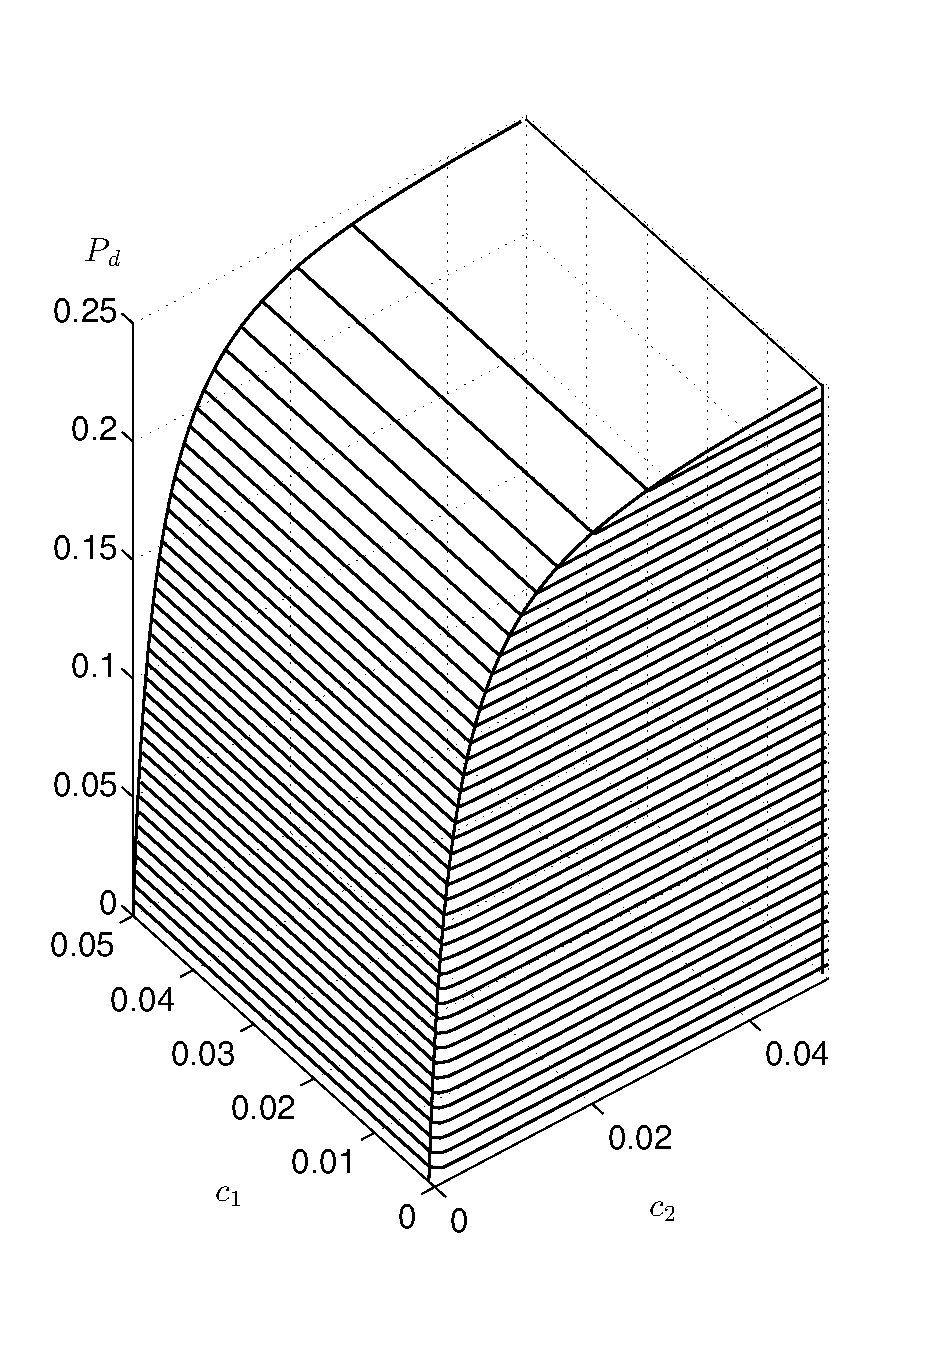
\includegraphics[width=12cm, height=16cm]{4/ROCsurface.eps}
  \caption{M-ROC surface for cyclostationary detector.}
  \label{pic:1221n0}
\end{figure}

\subsection{Simulation Results}
The simulation results presented in this thesis were obtained by using Monte Carlo techniques. In the simulation results, the signal are not affected by fading. All of Matlab code for the programs required to reproduce the simulation results are contained in the attached CD. Appendix B presents a brief tutorial on the uses of the various files for the simulation. 

Assume signal $s_A$ $s_B$ are OFDM signals with $16$ subcarriers ($l_D = 16$) and the length of the CP part is $\frac{1}{4}$ of the useful symbol data (in 802.11a standard, the CP part is also 1/4 length of the useful symbol data  \cite{1000232}). 
The subcarrier modulation employed QPSK. Similar to numerical analysis, let $K=50$, $\sigma_{s_A}^2 = 0.18$, $\sigma_{s_B}^2 = 0.15$ and $\sigma_{n}^2 = 0.3$. 
  
Since $l_D$ is not large, we cannot assume the OFDM signals to be governed by i.i.d. Gaussian distribution. This is different from the theoretical analysis, thus it may induce deviation between the simulation results and the numerical results. In reality, $l_D$ is usually a much larger number, e.g. in 802.11a standard, $l_D = 64$ \cite{1000232} and  in DVB-T standard, $l_D = 8192$ \cite{lunden2010robust}, in such situations the deviation between the numerical analysis and the simulation results will be smaller than that in this example.

The simulation presents the performance of cyclostationary detector when $c_1$ and $c_2$ separately increase from $0.005$ to $0.2$ with steps $0.005$. For a specified $c_1$ and $c_2$, we utilize Qian's algorithm of section 2.5 to calculate its MENP parameters $k_1$, $k_2$.

For each decision rule calculated through Qian's algorithm, we use Monte Carlo simulation to get its associated $P_d$, $P_{f_1}$ and $P_{f_2}$.   
In order to ensure highly accurate results, a minimum of 1000 events and 400000 experiments are required. The simulation result of the M-ROC surface is presented in Figure \ref{pic:15may09a1}. $P_d$ is acquired through simulation for each intersection of the mesh in Figure \ref{pic:15may09a1}, except for points $c_1 = 0$, $c_2$ and $c_1$, $c_2 = 0$, which are plotted to better illustrate the M-ROC surface. 
Compare Figure \ref{pic:15may09a1} with Figure \ref{pic:1221n0}, we can see the simulation result accords with the numerical analysis, i.e. the deviation brought by the mismatch between the mathematical model and the practice signals is negligible.
 
Figure \ref{pic:15may10a1} depicts the relationship between  $P_d$ and $k_1$ $k_2$ ($k_1$, $k_2$ are MENP parameters computed through Qian's algorithm of section 2.5).
For each $c_1, c_2$, the associated $(k_1, k_2, P_d)$ is plotted as `o'. The curve in Figure \ref{pic:15may10a1} is the theoretical relationship between $P_d$ and $k_1$, $k_2$. It is calculated through \eqref{equ: pf and pd}. Figure \ref{pic:15may10a2} is the projection of Figure \ref{pic:15may10a1} on $k_1-k_2$ plane.
In Figure \ref{pic:15may10a1}, we does not plot the theoretical $P_d$ for point A (with coordinate $(k_1, k_2, P_d) = (7.030, 7.031, 0.7388)$). Substitute $(k_1, k_2) = (7.030, 7.031)$ into \eqref{equ: pf and pd} we get the theoretical $P_d$ for point A is $0.7384$. Thus we can see for point A, the difference between theoretical $P_d$ and simulation $P_d$ is very small. 
Since $c_1$ and $c_2$ are discrete, points $(k_1, k_2)$ are also discrete, which can be seen from Figure \ref{pic:15may10a1} and Figure \ref{pic:15may10a2}. 
Furthermore, for different $(c_1, c_2)$, the value of $(k_1, k_2)$ may be the same, 
e.g. for $(c_1, c_2) = (0.1, 0.1)$, we have $k_1 = 0$ and $k_2  = 0.7568$; for $(c_1, c_2) = (0.2, 0.1)$, we have the same $k_1$ and $k_2$ value. 
In our program, we use Monte Carlo simulations to acquire the $P_d$ for each $(c_1, c_2)$.  For  $(c_1, c_2) = (0.1, 0.1)$, the $P_d$ we acquired is $0.9636$; for $(c_1, c_2) = (0.2, 0.1)$, the $P_d$ we acquired through simulation is $0.9635$. There are some slight difference between the two $P_d$ (even though the MENP parameters, so is the decision rule, are the same). This is because when the experiments times is not unlimited, the simulation results could be slightly different from each other. This explains why in Figure \ref{pic:15may10a1} for the same $(k_1, k_2)$, there may be multiple $P_d$ corresponds with it.  
We can also observe from Figure \ref{pic:15may10a1} and Figure \ref{pic:15may10a2} that except for point A, all other points either satisfy $k_1 = 0$ or $k_2 = 0$. This is reasonable. From the discussion in section 2.5 and in \cite{zhang2000efficient}, when $(c_1, c_2) \notin \alpha^+$, we have either $k_1 = 0$ or $k_2 = 0$. From Figure \ref{pic:1221n0}, we know region $M_0$ degenerates to a curve. Since $\alpha^+$ is the projection of $M_0$ on $c_1-c_2$ plane, it is easy to see set $\alpha^+$ also degenerates to a curve in $c_1-c_2$ plane. In our example, $c_1$ and $c_2$ increase from 0.005 to 0.2 with steps 0.2, it is plausible that only few $(c_1, c_2)$ lies in region $\alpha^+$. This explain why for most of the points in Figure \ref{pic:15may10a1} and Figure \ref{pic:15may10a2} we have either $k_1 = 0$ or $k_2 = 0$.
From Figure \ref{pic:15may10a1}, we can see even though there is some deviation between the mathematical model and the practice signals, the simulation results accords with the numerical results well. 

Figure \ref{pic:15may10a3} depicts the relationship between $P_{f_1}$, $P_{f_2}$ and $P_d$ for each decision rule computed through Qian's algorithm.  
For each $c_1, c_2$, the associated $(P_{f_1}, P_{f_2}, P_d) $ is plotted as `o'.
The curve in Figure \ref{pic:15may10a3} is the theoretical relationship between $P_{f_1}$ $P_{f_2}$ and $P_d$. This curve is computed through \eqref{equ: pf and pd}. 
As we have discussed, for one decision rule, there could be multiple simulation results for $(P_{f_1}, P_{f_2}, P_d)$, and these simulation results may be slight different due to the experiments times' limitation. 
This explains why in Figure \ref{pic:15may10a3} for some $(P_{f_1}, P_{f_2}, P_d)$ points, there are several  `o' near the theoretical curve.
By comparing the simulation results and the theoretical curve, we can see the simulation result accords with the numerical analysis. 

From the above analysis we can see even though there are some mismatch between the mathematical model and the practice signals, the simulation results still accords with the numerical results. In reality, e.g. 802.11a standard or DVB-T standard, the subcarrier number is much larger than 16, hence the difference between the numerical results and the simulation results should be  smaller. 


\begin{figure}[!t]
  \centering 
  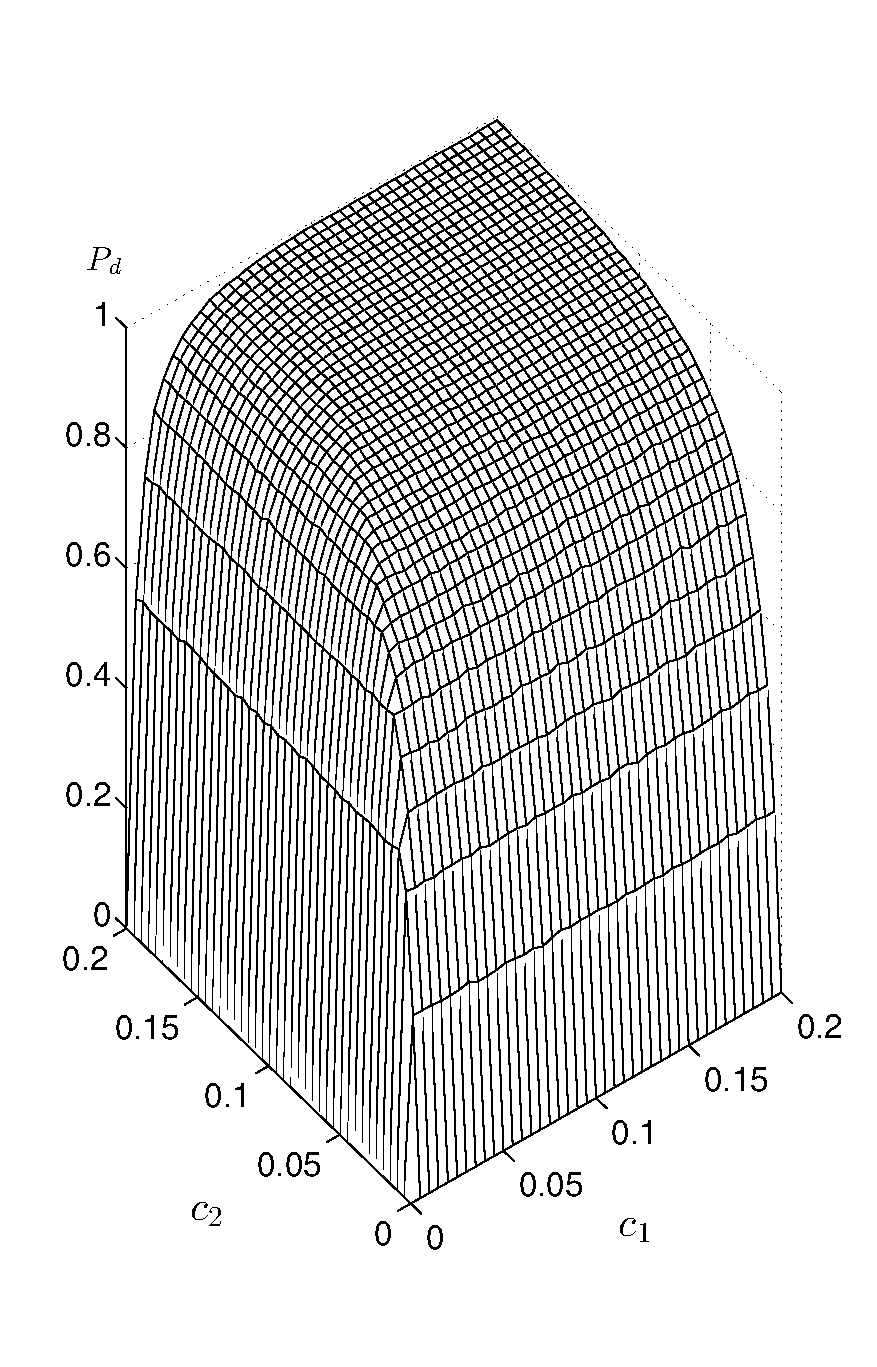
\includegraphics[width=12cm, height=16cm]{4/Cyc1c2pd.eps}
  \caption{Simulation results of M-ROC surface for cyclostationary detector.}
  \label{pic:15may09a1}
\end{figure}

\begin{figure}[!t]
  \centering 
  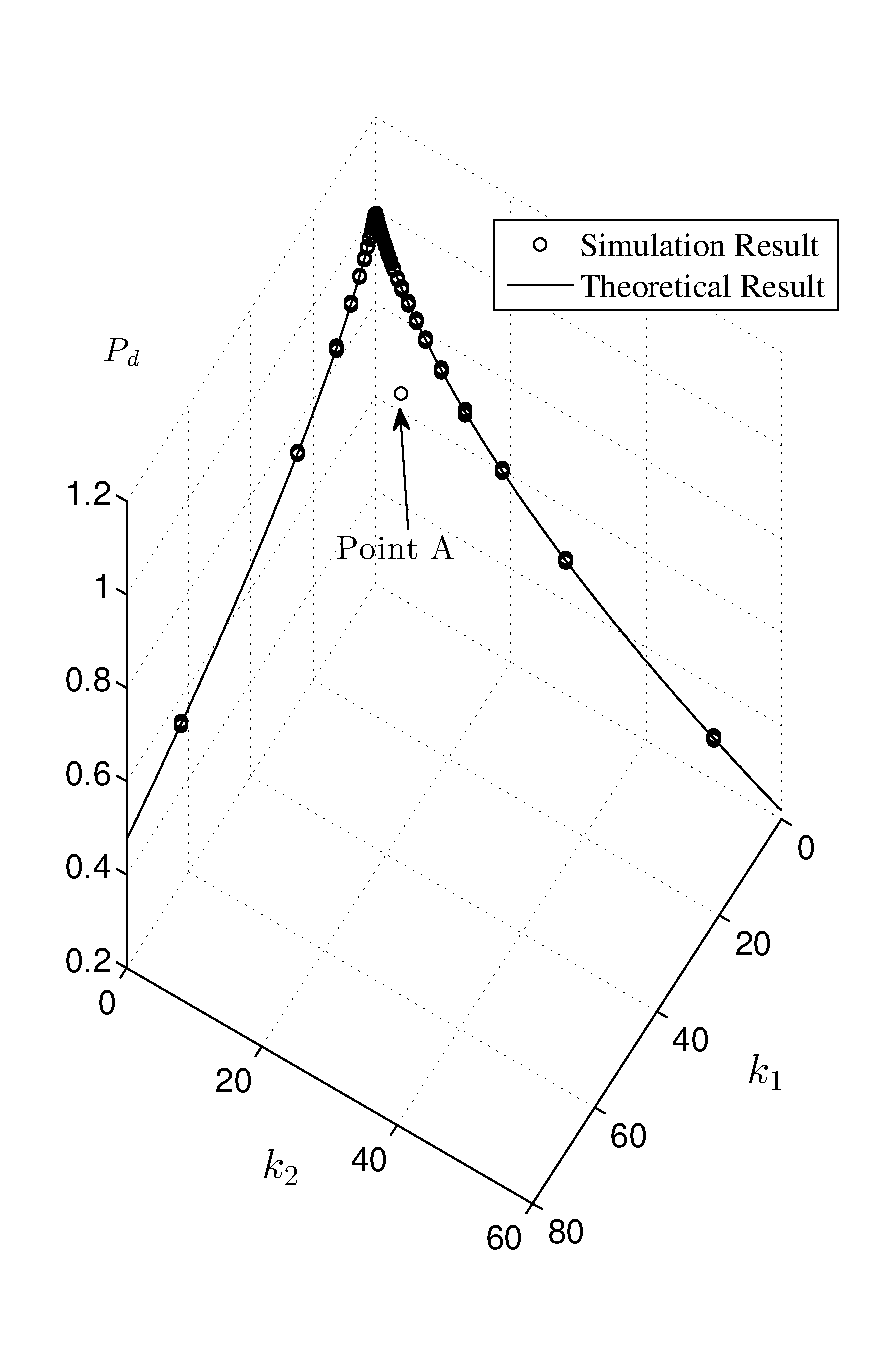
\includegraphics[width=12cm, height=16cm]{4/k1k2pd.eps}
  \caption{Relationship between $k_1$, $k_2$ and $P_d$.}
  \label{pic:15may10a1}
\end{figure}

\begin{figure}[!t]
  \centering 
  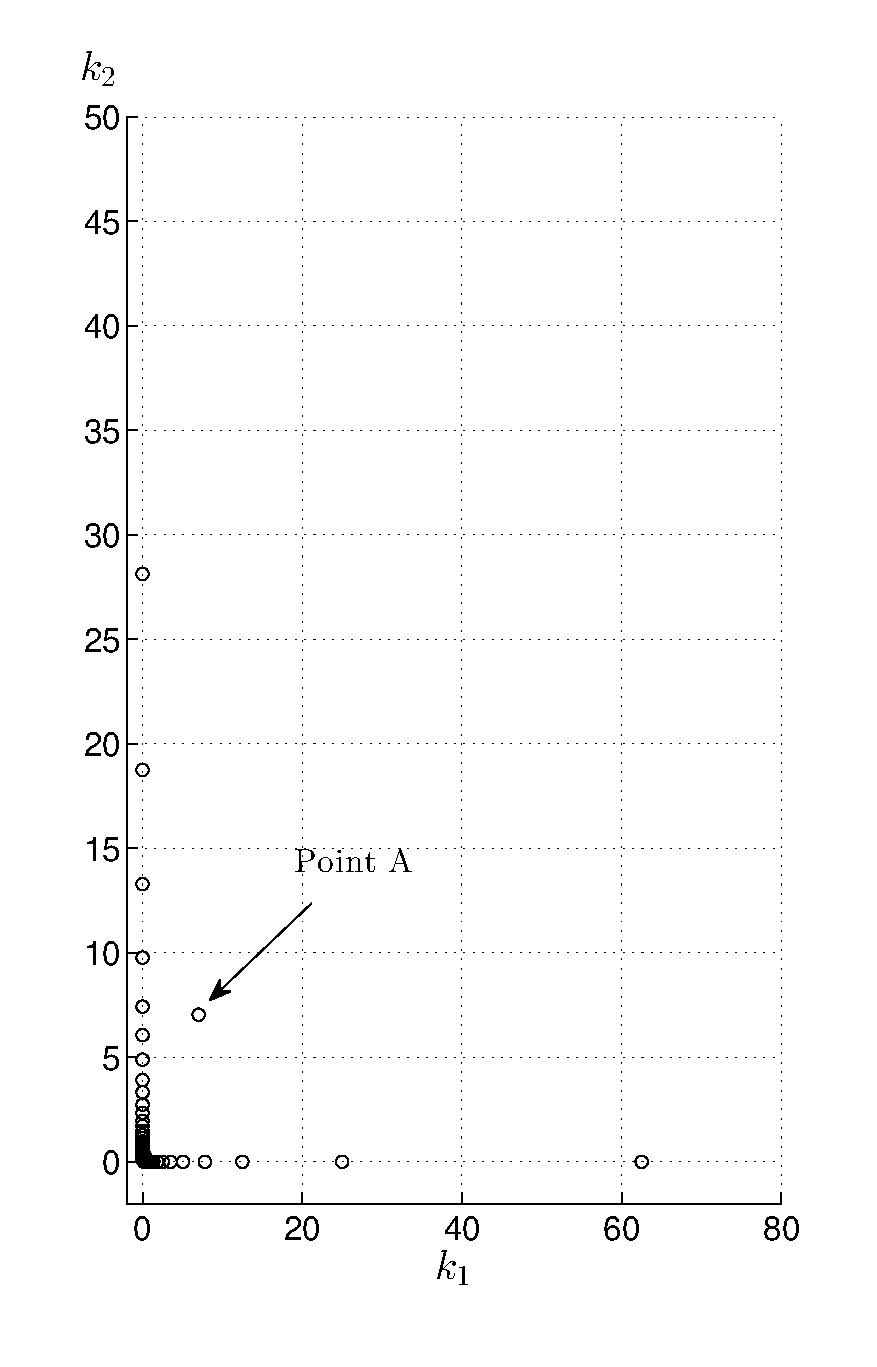
\includegraphics[width=12cm, height=16cm]{4/k1k2.eps}
  \caption{MENP parameters calculated through Qian's algorithm.}
  \label{pic:15may10a2}
\end{figure}

\begin{figure}[!t]
  \centering 
  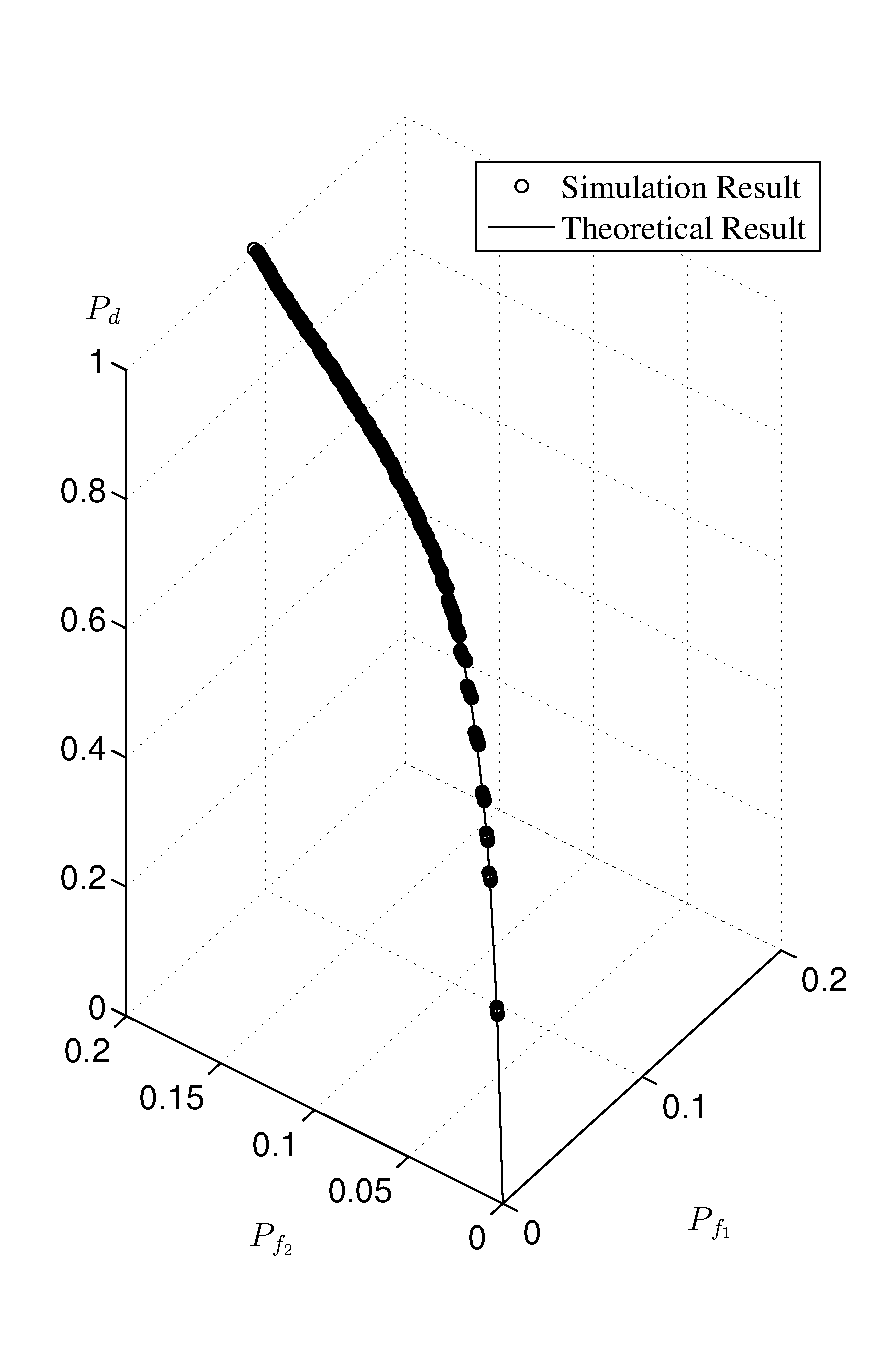
\includegraphics[width=12cm, height=16cm]{4/Cypf1pf2pd.eps}
  \caption{Relationship between $P_{f_1}$, $P_{f_2}$ and $P_d$.}
  \label{pic:15may10a3}
\end{figure}
